\documentclass[12pt,a4paper]{article}

% Paquetes básicos
\usepackage[utf8]{inputenc}
\usepackage[T1]{fontenc}
\usepackage{lmodern}
\usepackage[spanish]{babel}
\usepackage{amsmath, amssymb}
\usepackage{siunitx} % Ángulos
\usepackage{graphicx}
\usepackage{float}
\usepackage{geometry}
\usepackage{xcolor}
\geometry{margin=2.5cm}
\usepackage{hyperref}
\usepackage{caption}
\usepackage{subcaption}
\usepackage{setspace}
\usepackage{multirow}
\usepackage{minted}  % Códigos
\usepackage{gensymb} % Grados: "°"
\usepackage[backend=biber, style=ieee]{biblatex}
\addbibresource{Bibliografía.bib}
\graphicspath{{Figuras/}}
\onehalfspacing
\hypersetup{
    colorlinks  = true,
    linkcolor   = blue,    
    citecolor   = blue,
    urlcolor    = blue,
    filecolor   = blue
}


\begin{document}       
\renewcommand{\figureautorefname}{Fig.}
\renewcommand{\tableautorefname}{Tab.}
\renewcommand{\equationautorefname}{Ec.}


% Carátula personalizada
\begin{titlepage}
    \centering
    
\includegraphics[width=0.25\textwidth]{escudo.png} 
    \hspace{1cm}
    
\includegraphics[width=0.3\textwidth]{download.png} \\[1cm]

    {\large \textbf{UNIVERSIDAD NACIONAL DE CÓRDOBA} \\[0.5cm]}
    {\large \textbf {FACULTAD DE CIENCIAS EXACTAS, FÍSICAS Y NATURALES} \\[1cm]}
    {\Large ELECTRÓNICA INDUSTRIAL \\[1cm]}

    \rule{\textwidth}{0.5pt} \\[0.5cm]
    {\Large \textbf{TRABAJO FINAL DE INTEGRACIÓN:} \\[0.3cm]}
    {\Large \textbf{Conversor Boost Dual Trifásico (DC-DC)} \\[0.3cm]}
    {\Large \textbf{para Aplicaciones Fotovoltaicas} \\[0.3cm]}
    \rule{\textwidth}{0.5pt} \\[1cm]
    
\begin{tabular}{l l}
\textbf{Profesor Titular:} & Ing. Agüero Adrián. \\
\\
\textbf{Alumnos:} & Mendes Rosa, Agustín (44.517.201)\\
                  & Monja, Ernesto Joaquín (43.873.728)\\
\end{tabular}\\[3cm]

{\centering Año 2026 \par}

\end{titlepage}



% Índice
\tableofcontents
\newpage
\indent



\section{Introducción}                                                      \label{sec_1}
Hoy en día, la demanda global de energía eléctrica se encuentra en un constante y acelerado crecimiento, lo que plantea una búsqueda de diversificar la matriz energética y buscar alternativas para aprovechar las fuentes de energía renovable. Dentro de las energías renovables, la energía solar captada por paneles fotovoltaicos destaca como una opción viable y en constante expansión.

Uno de los problemas fundamentales de los paneles solares es que no entregan ni potencia, ni tensión, ni corriente constante tal como muestran las curvas características $I$-$V$ y $P$-$V$ de los mismos, ya que dependen de una multitud de factores ambientales tales como la temperatura, la hora del día, que tan despejado este el mismo, etcétera. Podemos ver estas variaciones en las curvas características de un Panel Solar típico del mercado, como lo puede ser el STP545S-B72/Pnh+, según la \autoref{fig:fig_1}:
\begin{figure}[H]
    \centering
    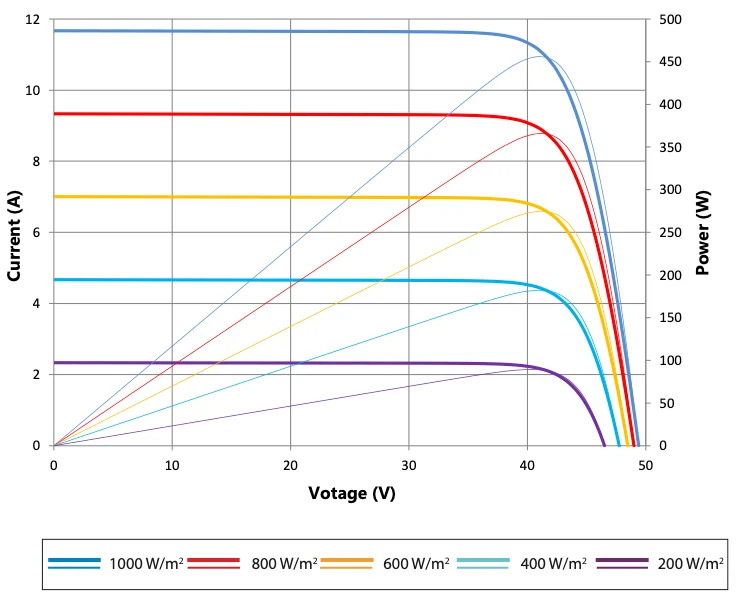
\includegraphics[width=0.8\linewidth]{Figura 1.png}
    \caption{Curvas $I$-$V$ y $P$-$V$ de un Panel Solar STP545S-B72/Pnh+.~\cite{b1}} 
    \label{fig:fig_1}
\end{figure}

Se tiene entonces que para compensar estas variaciones y lograr que el sistema opere en un punto de trabajo deseado, resulta indispensable la utilización de convertidores electrónicos de potencia tales como el \textit{Dual Three-Phase Boost Converter} (\textit{Convertidor Boost Dual Trifásico} traducido al Español), el cual podemos apreciar su topología circuital en la \autoref{fig:fig_2}.
\begin{figure}[H]
    \centering
    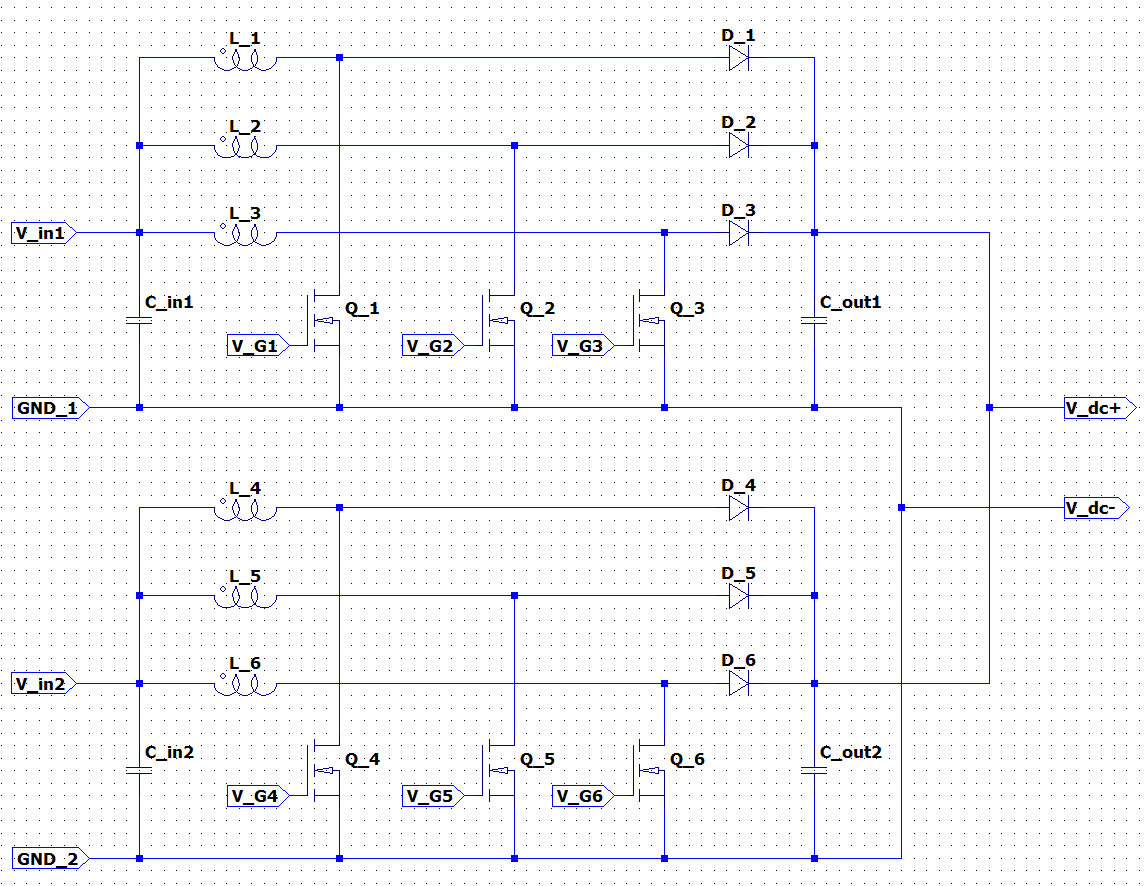
\includegraphics[width=0.8\linewidth]{Figura 2.png}
    \caption{Circuito Esquemático del Convertidor Dual Boost Trifásico.} 
    \label{fig:fig_2}
\end{figure}

Se tiene entonces que el objetivo principal de este \textit{Trabajo Final de Integración} consiste en estudiar, analizar, diseñar y simular un convertidor de esta topología enfocado en la conversión \textit{DC-DC} en aplicaciones fotovoltaicas, de acuerdo a los siguientes datos de diseño:
\begin{itemize}
    \item \underline{Tensión de entrada:} $48 \ [V_{DC}]$
    \item \underline{Tensión se salida:} $400 \ [V_{DC}]$
    \item \underline{Rango de corriente:} $0$ a $40 \ [A]$
\end{itemize}



\section{Desarrollo}                                                        \label{sec_2}
\subsection{Marco Teórico}                                                  \label{sec_2.1}
\subsubsection{Análisis del Convertidor Boost Monofásico}                   \label{sec_2.1.1}
El \textit{Convertidor Boost Monofásico}, como bien indica su nombre, tiene como función principal obtener a la salida del mismo, una tensión promedio de \textit{DC} mayor a la tensión de entrada, de modo que se dice que este ''eleva'' (\textit{Boost} del Inglés) la tensión de salida con respecto a la de entrada. El circuito básico consta de un Inductor ($L$), un interruptor controlado (típicamente un \textit{MOSFET} de potencia), un Diodo ($D$) y un Capacitor de Entrada ($C_{in}$) y de Salida ($C_{out}$) tal como el que se muestra en la \autoref{fig:fig_3}.
\begin{figure}[H]
    \centering
    
\includegraphics[width=0.8\linewidth]{Figura 3.png}
    \caption{Circuito Esquemático del Convertidor Boost Monofásico.} 
    \label{fig:fig_3}
\end{figure}

Nótese que el \textit{Convertidor Boost Dual Trifásico} presentado en la \autoref{fig:fig_2}, se trata de una topología derivada del \textit{Convertidor Boost Monofásico}, ya que en términos estructurales: Este convertidor está compuesto por 2 módulos idénticos conectados en paralelo, donde cada módulo es a su vez, un Convertidor Boost de 3 fases (3 ramas en paralelo). Esto significa que la potencia eléctrica del panel fotovoltaico fluye a través de 6 ramas independientes para entregar 2 valores de \textit{DC}, explicitados en la \autoref{fig:fig_2} como $V_{DC+}$ y $V_{DC-}$~\cite{b2}. Se tiene entonces que si se desea diseñar un \textit{Convertidor Boost Dual Trifásico}, resulta fundamental comenzar el estudio por su par monofásico.

El principio de funcionamiento del \textit{Convertidor Boost Monofásico} se basa en el almacenamiento de energía magnética en el Inductor $L$, el cual se carga y descarga mediante el accionar de una llave electrónica, que por lo general consiste de un \textit{MOSFET}. Para entender mejor su funcionamiento y basándonos en la \autoref{fig:fig_3}, veamos que ocurre en el circuito cuando el transistor $Q$ esta en un estado u otro:
\begin{itemize}
    \item \underline{Estado 1 - Interruptor Cerrado ($ON$):} Cuando el \textit{MOSFET} entra en conducción, el inductor queda conectado en paralelo con la fuente de alimentación ($V_{in}$ en nuestro esquemático). Durante este intervalo, la corriente que atraviesa el inductor aumenta de forma lineal, almacenando energía en su campo magnético. Simultáneamente, el diodo queda polarizado en inversa, desconectando la etapa de entrada de la carga. En este instante, es el capacitor de salida el encargado exclusivo de suministrar la corriente y mantener la tensión en la carga.
    
    \item \underline{Estado 2 - Interruptor Abierto ($OFF$):} Al abrirse el \textit{MOSFET}, la corriente del inductor no puede interrumpirse de forma instantánea. Por lo tanto, la polaridad de la tensión en el inductor se invierte para mantener el flujo de corriente, sumándose a la tensión de la fuente de entrada. Esta acción polariza el diodo en directa, permitiendo que la energía almacenada en el inductor, junto con la proporcionada por la fuente, fluya hacia la etapa de salida para alimentar la carga y recargar el capacitor.~\cite[págs. 172-178]{b3}
\end{itemize}

Luego se tiene que las formas de onda características de este circuito son las que se presentan en la \autoref{fig:fig_4}.
\begin{figure}[H]
    \centering
    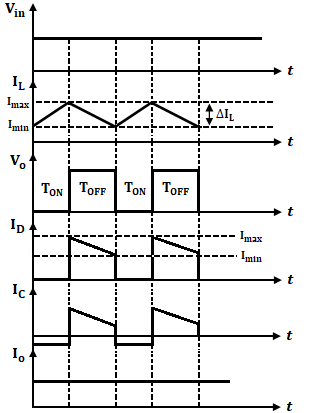
\includegraphics[width=0.5\linewidth]{Figura 4.png}
    \caption{Formas de Onda del \textit{Convertidor Boost Monofásico}.~\cite{b4}} 
    \label{fig:fig_4}
\end{figure}

Los ejes verticales de la \autoref{fig:fig_4}, se corresponden a los siguientes valores relacionados al esquemático planteado en la \autoref{fig:fig_3}:
\begin{itemize}
    \item \underline{$I_{L}$:} Es la corriente a través del Inductor $L$.
    \item \underline{$V_{0} = V_{out}$:} Es la tensión de salida del Convertidor.
    \item \underline{$I_{D}$:} Es la corriente a través del Diodo $D$.
    \item \underline{$I_{C}$:} Es la corriente a través del Capacitor $C_{out}$.
    \item \underline{$I_{0} = I_{out}$:} Es la corriente de salida del Convertidor.
\end{itemize}



\subsubsection{Ecuaciones de Diseño}                                        \label{sec_2.1.2}
Si bien el convertidor a diseñar se trata de un \textit{Boost Dual Trifásico}, dado lo mencionado en la \autoref{sec_2.1.1}, es posible no tan solo tomar el principio de funcionamiento del \textit{Boost Monofásico}, sino también reutilizar las ecuaciones de diseño con el fin de calcular un único \textit{Boost Monofásico} y replicar su diseño y cálculos para las otras 5 ramas, logrando así los requerimientos especificados en la \autoref{sec_1}.

En cuanto a las ecuaciones de diseño de un \textit{Convertidor Boost Monofásico}, se opta en este informe utilizar como referencia el marco teórico presentado por la nota de aplicación de \textit{Texas Instruments}~\cite{b5}, la cual planta de forma detallada, una serie de pasos con ecuaciones para elegir correctamente los componentes, los cuales se presentan a continuación de forma resumida:
\begin{itemize}
    \item \underline{Paso 1 - Definición de los Datos de Diseño:} La nota de aplicación indica que se deben definir los siguientes parámetros antes de comenzar a calcular componentes:
    \begin{itemize}
        \item Mínima tensión nominal de entrada ($V_{in(min)}$).
        \item Tensión nominal de salida ($V_{out}$).
        \item Máxima corriente de salida ($I_{out(max)}$).
        \item Circuito integrado que actúa como llave electrónica, utilizado para construir el Convertidor Boost. Este paso es necesario ya que ciertos parámetros de los pasos posteriores requeriran de la hoja de datos del mismo. En este caso, trabajaremos con un \textit{MOSFET}.
    \end{itemize}


    \item \underline{Paso 2 - Calculo del Ciclo de Trabajo ($D$):} Para un \textit{Convertidor Boost}, se tiene que el ciclo de trabajo está definido en términos generales según la \autoref{eq_1}.~\cite[págs. 172-178]{b3}
    \begin{equation}
        V_{out} = \frac{V_{in}}{1 - D}
        \label{eq_1}
    \end{equation}
    La nota de aplicación propone introducir una variable más denominada: $\eta$, siendo esta la eficiencia del convertidor y la estima en: $\eta \approx 80 \ [\%]$ como un valor aceptable para este tipo de convertidor. Por lo tanto, despejando a $D$ de la \autoref{eq_1} y asumiendo que la tensión de entrada es mínima (es decir que: $V_{in} = V_{in(min)}$), se tiene que:
    \begin{equation}
        D = 1 - \frac{V_{in(min)} \times \eta}{V_{out}}
        \label{eq_2}
    \end{equation}


    \item \underline{Paso 3 - Calculo del $\Delta I_{L}$:} Esta consiste en la variación de la corriente que ocurre en el inductor tal como se observa en la \autoref{fig:fig_4}. Para ello el fabricante la estima como un porcentaje de la corriente máxima de salida según la \autoref{eq_3}.
    \begin{equation}
        \Delta I_{L} = (0.2 \text{ a } 0.4) \times I_{out(max)} \times \frac{V_{out}}{V_{in}}
        \label{eq_3}
    \end{equation}


    \item \underline{Paso 4 - Calculo de la Inductancia ($L$):} Si el fabricante del circuito integrado de conmutación no entrega en su hoja de datos un valor o rango indicado para esta inductancia, la nota de aplicación provee la \autoref{eq_4} como una buena estimación para la inductancia.
    \begin{equation}
        L = \frac{V_{in} \times (V_{out} - V_{in})}{\Delta I_{L} \times f_{s} \times V_{out}}
        \label{eq_4}
    \end{equation}
    Donde $f_{S}$ es la frecuencia mínima de conmutación del Convertidor.


    \item \underline{Paso 5 - Calculo de la Corriente Máxima del Interruptor ($I_{SW(max)}$):} Esta es la corriente pico que debe soportar la llave electrónica, la cual en nuestro caso al tratarse de un \textit{MOSFET}, se refiere a la $I_{D}$~\cite{b6}. Esta corriente se determina entonces según la \autoref{eq_5}
    \begin{equation}
        I_{SW(max)} = \frac{\Delta I_{L}}{2} + \frac{I_{out(max)}}{1 - D}
        \label{eq_5}
    \end{equation}


    \item \underline{Paso 6 - Selección del Diodo ($D$):} La nota de aplicación recomienda utilizar
    diodos Schottky para reducir las perdidas e indica que la corriente directa de selección debe ser igual a la corriente máxima de salida, es decir:
    \begin{equation}
        I_{F(AV)} = 1.3 \times I_{out(max)}
        \label{eq_6}
    \end{equation}
    Se incluyo en la \autoref{eq_6} un coeficiente de seguridad del $30 [\%]$ para elegir esta corriente~\cite[Pág. 22]{b7}. Adicionalmente, se indica que otro parámetro que debe ser tenido en cuenta es que la potencia de disipación del diodo debe soportar:
    \begin{equation}
        P_{D} = V_{F} \times I_{F}
        \label{eq_7}
    \end{equation}
    

    \item \underline{Paso 7 - Selección del Capacitor de Salida Mínimo ($C_{out(min)}$):} Esta capacitancia depende del ripple de tensión de salida deseado ($\Delta V_{out}$) y la nota recomienda que se calcule según la \autoref{eq_8}.
    \begin{equation}
        C_{out(min)} = \frac{I_{out(max)} \times D}{f_{s} \times \Delta V_{out}}
        \label{eq_8}
    \end{equation}
\end{itemize}

Nótese que el único valor que no se ha calculado ha sido el Capacitor de Entrada ($C_{in}$) ya que la nota de aplicación indica que el valor mínimo para el capacitor de entrada esta normalmente dado en la hoja de datos del circuito integrado de conmutación~\cite{b5}. Dado que la llave electrónica esta implementada mediante un \textit{MOSFET}, no es factible depender de si la hoja de datos del \textit{MOSFET} elegido, incluya como aplicación un \textit{Convertidor Boost} y que a su vez contemple la existencia de $C_{in}$ (Nótese que un \textit{Convertidor Boost} no necesariamente tiene que ser utilizado en aplicaciones fotovoltaicas como la nuestra, donde la tensión de entrada no es constante, y por lo tanto no existe motivo para introducir un capacitor a la entrada).

Para solventar este problema, se recurre al análisis de la forma de onda de la corriente de entrada $I_{in}$ la cual es la misma que la corriente a través del inductor $L$, ya que se trata de la misma rama~\cite{b8}. Se tiene que según la \autoref{fig:fig_4}, la corriente del inductor ($I_{L}$) tiene una forma de onda triangular con un valor medio ($I_{in}$) y un rizado pico a pico ($\Delta I_L$).

La función del capacitor de entrada ($C_{in}$) es absorber la parte alterna (el rizado triangular) de esa corriente, dejando que a la fuente (los paneles) solo le llegue la corriente continua. Por otro lado, se sabe que la variación de tensión en un capacitor ($\Delta V$) está dada por la cantidad de carga eléctrica ($\Delta Q$) que acumula.
\begin{equation}
    \Delta V_{in} = \frac{\Delta Q}{C_{in}} \rightarrow C_{in} = \frac{\Delta Q}{\Delta V_{in}}
    \label{eq_9}
\end{equation}

La cantidad de carga eléctrica ($\Delta Q$) es el área del triángulo de corriente durante la mitad del ciclo en la que la corriente está por encima de cero es decir, cuando el capacitor se está cargando~\cite{b8}. Se tiene que el área de este triangulo estará dada por:
\begin{itemize}
    \item La base de ese triángulo es la mitad del período de conmutación: $b = \frac{T_s}{2}$.
    \item La altura de ese triángulo es la mitad del rizado pico a pico: $h = \frac{\Delta I_L}{2}$.
\end{itemize}

Por lo tanto, se tiene que el área de este triángulo estará dada por:
\begin{equation}
    Area = \frac{b \times h}{2} \rightarrow \Delta Q = \frac{1}{2} \times \left(\frac{T_{s}}{2}\right) \times \left(\frac{\Delta I_L}{2}\right) = \frac{\Delta I_L \times T_s}{8} 
    \label{eq_10}
\end{equation}

Sabiendo que el período $T_{s}$ es la inversa de la frecuencia ($T_{s} = \frac{1}{f_{s}}$), la ecuación de la carga queda:
\begin{equation}
    \Delta Q = \frac{\Delta I_{L}}{8 \times f_{s}}
    \label{eq_11}
\end{equation}

Se tiene que finalmente reemplazando lo obtenido en la \autoref{eq_11} en la \autoref{eq_9}, se tiene que:
\begin{equation}
    C_{in} = \frac{\Delta I_{L}}{8 \times f_{s} \times \Delta V_{in}}
    \label{eq_12}
\end{equation}



\subsection{Diseño del Conversor Boost Dual Trifásico}                      \label{sec_2.2}
\subsubsection{Calculo de una rama Boost Monofásico}                        \label{sec_2.2.1}
Tal como se menciono en la \autoref{sec_2.1.2}, se busca diseñar un único \textit{Convertidor Boost Monofásico} y replicar su diseño otras 5 veces, de modo que al estar los 6 módulos en paralelo, se obtenga el \textit{Convertidor Boost Dual Trifásico} con las características deseadas.

Se tiene entonces que al utilizar una topología de 6 ramas en paralelo, donde cada rama individual representa un \textit{Convertidor Boost Monofásico} la cual deberá manejar una sexta parte de la corriente total. Con esta consideración en mente, podemos comenzar con el proceso de selección de acuerdo a los pasos listados en la \autoref{sec_2.1.2}.
\begin{itemize}
    \item \underline{Paso 1:} Los parámetros de diseño de cada convertidor son:
    \begin{itemize}
        \item $V_{in(min)} = 48 \ [V]$.
        \item $V_{out} = 400 \ [V]$.
        \item $I_{out(max)} = \frac{40 \ [A]}{6} \approx 6.67 \ [A]$.
    \end{itemize}
    El resto de parámetros se irán definiendo en los pasos posteriores.


    \item \underline{Paso 2:} Según la \autoref{eq_2}, se tiene que:
    \begin{equation}
        D = 1 - \frac{48 \times 0.8}{400} = 90.4 \ [\%]
        \label{eq_13}
    \end{equation}


    \item \underline{Paso 3:} Tomando un $30 \ [\%]$ de la corriente máxima, se determina según \autoref{eq_3} que el ripple de corriente en el inductor será de:
    \begin{equation}
        \Delta I_{L} = 0.3 \times (6.67) \times \left(\frac{400}{48}\right) = 16.675 \ [A]
        \label{eq_14}
    \end{equation}


    \item \underline{Paso 4:} Para determinar el valor de la inductancia $L$, debemos primero fijar una frecuencia mínima de conmutación, la cual depende de forma directa del elemento encargado de la conmutación que en este caso, se trata de un \textit{MOSFET}.

    Según lo desarrollado en la \autoref{sec_2.1.2} (más específicamente las \autoref{eq_4}, \autoref{eq_8} y la \autoref{eq_12}), la selección de la frecuencia de conmutación ($f_{s}$) representa un compromiso directo entre el volumen de los componentes reactivos y las pérdidas por conmutación en los semiconductores~\cite[Cap. 4, Sec. 3]{b8}. Se tiene que dado que se trata de una topología de $N = 6$ ramas, el sistema se beneficia de una frecuencia efectiva de:
    \begin{equation}
        f_{efectiva} = N \times f_{s}
        \label{eq_15}
    \end{equation}

    Dadas las ventajas constructivas físicas del \textit{MOSFET}, se tiene que este permite trabajar con frecuencias de conmutación mucho más altas que las de los IGBTs~\cite[pág. 20]{b9}~\cite{b10}, sin embargo para este tipo de aplicaciones, se utilizan otros tipos de \textit{MOSFETs} los cuales se discutirán en secciones posteriores.
        
    Dada la topología de 6 ramas ($N = 6$), el sistema se beneficia de una frecuencia efectiva de $N \times f_{s}$. Esto permite seleccionar una $f_{s}$ conservadora por rama de $100 \ [kHz]$, garantizando una frecuencia efectiva de filtrado de $600 \ [kHz]$. Por lo tanto, si: $f_{s} = 100 \ [kHz]$, se tiene que reemplazando este valor en la \autoref{eq_4}, se tiene que:
    \begin{equation}
        L = \frac{48 \times (400 - 48)}{16.675 \times 100000 \times 400} \approx 25.33 \ [\mu Hy]
        \label{eq_16}
    \end{equation}
    
    
    \item \underline{Paso 5:} Este paso si bien no será utilizado en esta sección sino más bien en la posterior a esta, nos da un indicador de que tipo de \textit{MOSFET} deberemos utilizar, por lo tanto, reemplazando los valores obtenidos en los pasos anteriores en la \autoref{eq_5}
    \begin{equation}
        I_{SW(max)} = \frac{16.675}{2} + \frac{6.67}{1 - 0.904} \approx 77.81 \ [A]
        \label{eq_17}
    \end{equation}


    \item \underline{Paso 6:} Al igual que el paso anterior, este será utilizado en la sección posterior para elegir el diodo, tal que según la \autoref{eq_6}:
    \begin{equation}
        I_{F(AV)} = 1.3 \times 6.67 \approx 8.671 \ [A]
        \label{eq_18}
    \end{equation}


    \item \underline{Paso 7:} Para calcular al capacitor de salida, debemos primero fijar que ripple se permite a la salida, tal que tomando que este ripple sea del $1 \ [\%]$, lo que equivale a un:
    \begin{equation}
        \Delta V_{out} = 0.01 \times 400 = 4 \ [V]
        \label{eq_19}
    \end{equation}
    Tal que reemplazando lo obtenido en la \autoref{eq_19} en la \autoref{eq_8}, se obtiene la capacitancia de salida mínima.
    \begin{equation}
        C_{out(min)} = \frac{6.67 \times 0.904}{100000 \times 4} \approx 15.07 \ [\mu F]
        \label{eq_20}
    \end{equation}
    Se opta entonces por un capacitor de valor comercial de $C_{out} = 18 \ [\mu F]$.

    
    \item \underline{Paso 8:} Si bien no existe un paso 8 en la \autoref{sec_2.1.2}, se dirá que el paso 8 para nuestros cálculos consiste en determinar el capacitor de entrada ($C_{in}$) de acuerdo a la expresión de la \autoref{eq_12}. Para ello, solo resta determinar el ripple a la entrada, para el cual se toma el mismo criterio del $1 \ [\%]$ del paso anterior, tal que $\Delta V_{in} = 0.01 \times 48 = 0.48 \ [V]$ tal que:
    \begin{equation}
        C_{in} = \frac{16.675}{8 \times 100000 \times 0.48} \approx 43.42 \ [\mu F]
        \label{eq_21}
    \end{equation}
    Se elige entonces un capacitor de valor comercial de $C_{in} = 47 \ [\mu F]$.
\end{itemize}



\subsubsection{Selección de Componentes}                                    \label{sec_2.2.2}
En esta sección profundizaremos sobre el proceso de selección de los 2 elementos activos que conforman el \textit{Convertidor Boost}:
\begin{itemize}
    \item \textbf{Selección del MOSFET:} De acuerdo a lo discutido en la \autoref{sec_2.1.2}, si bien la llave electrónica a utilizar será un \textit{MOSFET} debido a que este ofrece las mejores velocidades de conmutación~\cite[pág. 20]{b9}~\cite{b10}, se tiene que las pérdidas de conmutación a una frecuencia de $f_{s} = 100 [kHz]$ y las altas tensiones y corrientes de trabajo, se descartó el uso de \textit{MOSFETs} convencionales de Silicio (\textit{Si}). 
    
    De acuerdo al artículo académico de \textit{Texas Instruments} sobre las perdidas en los \textit{MOSFETS}~\cite[Eq. 4]{b11}, las pérdidas por conmutación ($P_{SW}$) son directamente proporcionales a la tensión aplicada ($V_{IN}$), la corriente y la frecuencia de operación ($f_{SW}$), gobernadas de forma crítica por la carga de transferencia de compuerta ($Q_{GS2} + Q_{GD}$), según la expresión \autoref{eq_22}.
    \begin{equation}
        P_{sw} = V_{in} \times I_{out} \times f_{s} \times \frac{(Q_{GS2} + Q_{GD})}{I_{G}}
        \label{eq_22}
    \end{equation}
    
    Adicionalmente, las pérdidas asociadas a la carga de la compuerta ($P_{G}$) escalan linealmente con la frecuencia~\cite[Eq. 5]{b11} según la expresión \autoref{eq_23}.
    \begin{equation}
        P_{G} = Q_{G(TOT)} \times V_{G} \times f_{s}
        \label{eq_23}
    \end{equation}
    
    En transistores de \textit{Si} de alta tensión, la reducción de la resistencia en conducción ($R_{DS(on)}$) impone una penalización directa aumentando la capacitancia de compuerta, lo que ante una frecuencia de conmutación de $100 \ [kHz]$ elevaría exponencialmente las pérdidas dinámicas globales, tal como se muestra en la \autoref{fig:fig_5}
    \begin{figure}[H]
        \centering
        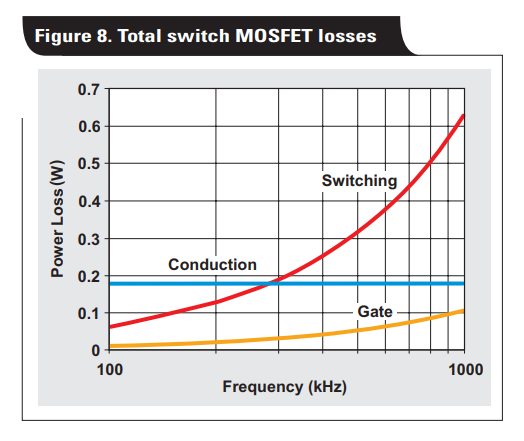
\includegraphics[width=0.5\linewidth]{Figura 5.png}
        \caption{Formas de Onda del \textit{Convertidor Boost Monofásico}.~\cite[Fig. 8]{b11}} 
        \label{fig:fig_5}
    \end{figure}
    
    Por este motivo, se justifica de forma crítica la transición hacia transistores de Carburo de Silicio (\textit{SiC})~\cite{b12}. Se tiene que según lo desarrollado en el Paso 5 de la \autoref{sec_2.2.1}, se tiene que los parámetros de elección de un este \textit{MOSFET} serán los siguientes:
    \begin{itemize}      
        \item \underline{Tensión Drenador-Surtidor ($V_{DS}$):} Se tiene que la máxima tensión que soportará el transistor es prácticamente la tensión de salida $V_{out} = 400 \ [V]$, multiplicada por un factor de seguridad de $2.5$ veces, tal que se debe elegir un \textit{MOSFET} con una tensión drenador-surtidor máxima de: $V_{DS} \approx 1000 \ [V]$.

        \item \underline{Corriente de Drenador ($I_{D}$):} De acuerdo a lo expresado en la \autoref{eq_17}, se tiene que se debe elegir un \textit{MOSFET} con una corriente de drenador máxima de: $I_{D} \approx 80 \ [A]$.
    \end{itemize}
    Se elige entonces como \textit{MOSFET}, un \textbf{Wolfspeed C3M0016120K}~\cite{b13} el cual según su hoja de datos posee las especificaciones listadas en la \autoref{fig:fig_6}.
    \begin{figure}[H]
        \centering
        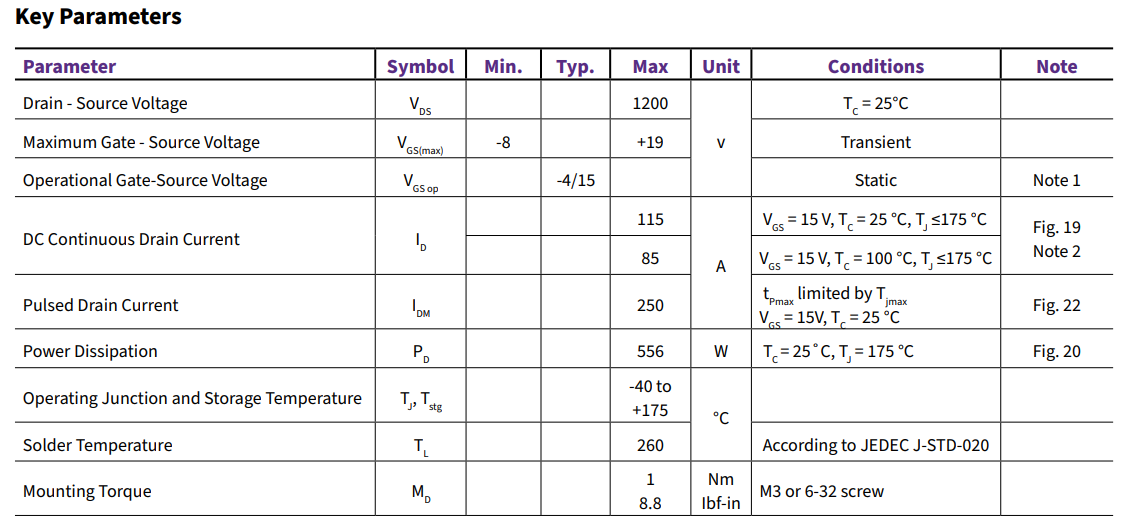
\includegraphics[width=0.9\linewidth]{Figura 6.png}
        \caption{Hoja de datos del Wolfspeed C3M0016120K.~\cite{b13}} 
        \label{fig:fig_6}
    \end{figure}


    \item \textbf{Selección del Diodo:} Si bien la nota de aplicación de \textit{Texas Instruments}, utilizada en la \autoref{sec_2.1.2}, recomienda utilizar diodos Schottky, se tiene que estos no existen para tensiones mayores a $150 \ [V]$ o $200 \ [V]$~\cite[Pág. 36]{b14}. Por lo tanto se recurre nuevamente a la tecnología de de Carburo de Silicio (\textit{SiC})~\cite{b12}, ya utilizada en los \textit{MOSFETs}, la cual presenta las mismas ventajas (altas tensiones y corrientes de trabajo en conjunto con altas frecuencias de conmutación) pero para Diodos Schottky. Se tiene entonces que los diodos se deben elegir según:~\cite[Págs. 19-21]{b14}
    \begin{itemize}
        \item \underline{Tensión Inversa Máxima ($V_{RRM}$):} Nótese que cuando el \textit{MOSFET} este encendido, el diodo queda polarizado en inversa y por consecuente, tiene que soportar toda la tensión de salida ($V_{out} = 400 \ [V]$). Aplicando el mismo coeficiente de seguridad que para el \textit{MOSFET}~\cite[pág. 22]{b7} y por lo tanto se elige el diodo según: $V_{RRM} \approx 1000 \ [V]$.

        \item \underline{Corriente directa Máxima de Conducción ($I_{F(AV)}$):} El diodo solo conducirá durante el tiempo que el \textit{MOSFET} este apagado, por lo tanto el diodo se debe elegir en base a la \autoref{eq_18}, es decir: $I_{F(AV)} = 9 \ [A]$.
    \end{itemize}
    En virtud de estos valores, se elige un diodo \textbf{Wolfspeed C4D20120D}~\cite{b15} el cual según su hoja de datos posee las especificaciones listadas en la \autoref{fig:fig_7}.
    \begin{figure}[H]
        \centering
        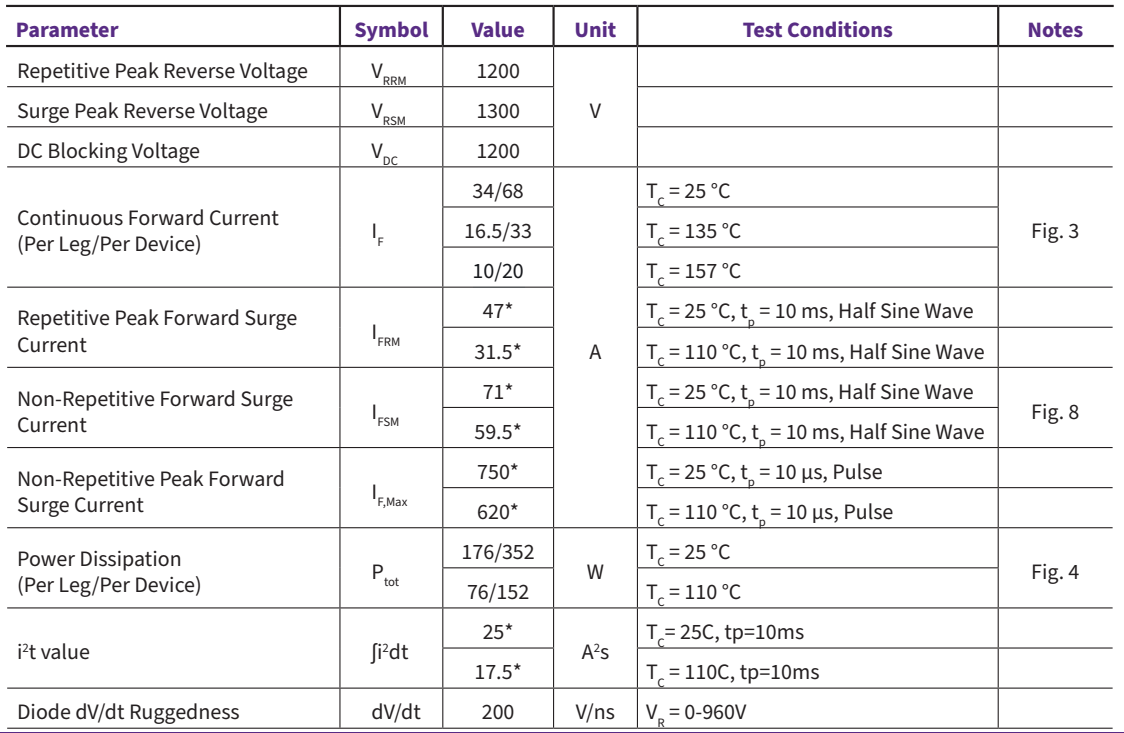
\includegraphics[width=0.75\linewidth]{Figura 7.png}
        \caption{Hoja de datos del Wolfspeed C4D20120D.~\cite{b15}} 
        \label{fig:fig_7}
    \end{figure}
\end{itemize}



\subsubsection{Simulación del Convertidor Boost Monofásico}                 \label{sec_2.2.3}
Se propone, dada la complejidad y cantidad de elementos que tiene el \textit{Convertidor Boost Dual Trifásico}, que se simule en una primera instancia el \textit{Convertidor Boost Monofásico} analizado y calculado en secciones anteriores. Una vez que esas simulaciones se correspondan con el diseño efectuado, se simulará el \textit{Convertidor Boost Dual Trifásico}. Nótese que a fines prácticos, la principal diferencia entre ambos va a ser la corriente de salida.

En virtud de lo recién mencionado, se tiene que el circuito a simular en LTSpice, se encuentra en representado en la \autoref{fig:fig_8}.
\begin{figure}[H]
    \centering
    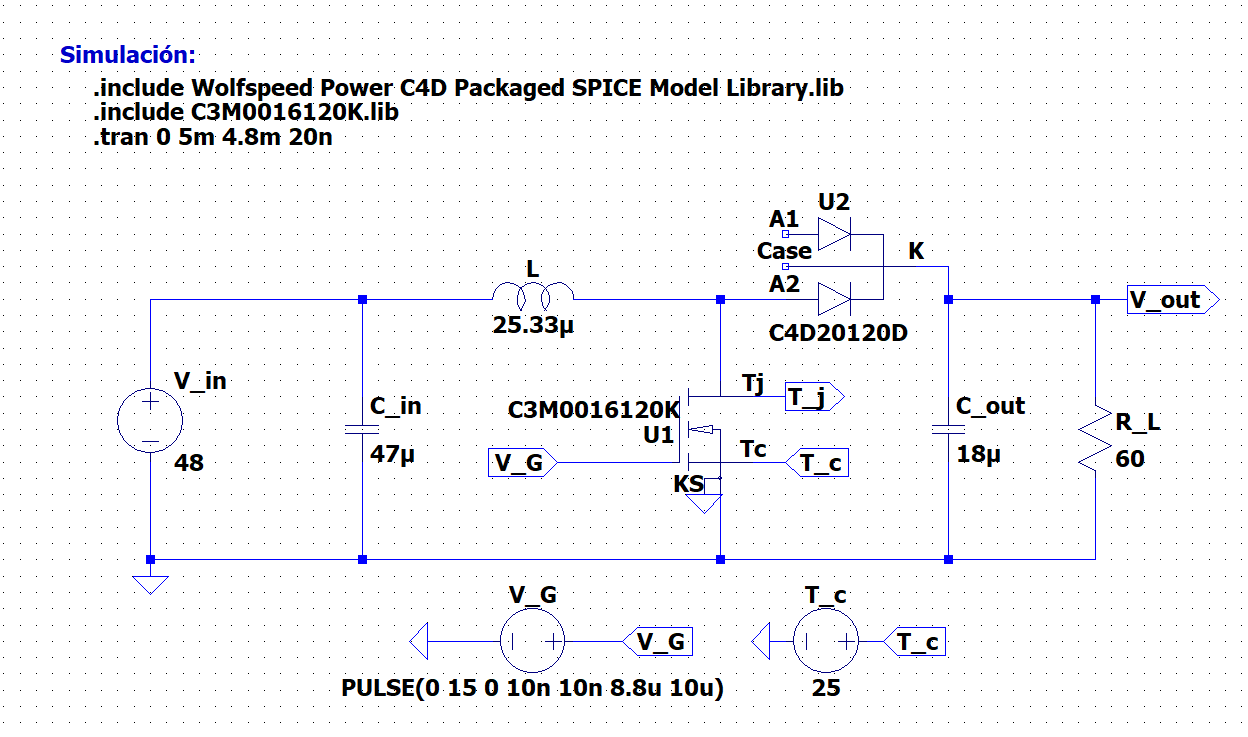
\includegraphics[width=0.75\linewidth]{Figura 8.png}
    \caption{Simulación en LTSpice del Convertidor Boost Monofásico.} 
    \label{fig:fig_8}
\end{figure}

Antes de observar los resultados de la simulación, se puede apreciar que los modelos de LTSpice tanto del Diodo \textbf{C4D20120D}, como del \textit{MOSFET} \textbf{C3M0016120K} se obtuvieron directamente de la página oficial de su fabricante, es decir, de \textbf{Wolfspeed}~\cite{b15}. El fabricante entrega no tan solo los modelos de simulación en archivos $.lib$, sino también que los archivos de los símbolos $.asy$ para introducirlos en el esquemático que se muestra en la \autoref{fig:fig_8}. Los modelos de LTSpice del para la simulación para el diodo y el \textit{MOSFET}, se encuentran en el \autoref{anex_A} y \autoref{anex_B} respectivamente.

Por otro lado, se puede observar que el modelo del \textit{MOSFET} incluye 2 terminales adicionales, denominados $T_{J}$ y $T_{C}$ los cuales se corresponden a la Temperatura de Juntura y de Carcasa del transistor. Estas variables pueden ser utilizadas como entradas (para introducir alguna temperatura inicial de trabajo) o como salidas (para medir la temperatura del transistor bajo carga). Estas
se modelan de acuerdo a la correspondencia de: $1 \ [V] \rightarrow 1 \ [\degree C]$ y para nuestro caso, se opto únicamente por fijar que :$T_{C} = 25 \ [\degree C]$.

A fines de realizar una simulación inicial, el disparo del \textit{MOSFET} será comandado por una fuente de tensión de pulsos ajustada a un ciclo de trabajo ($D$) similar al obtenido en la \autoref{eq_13}, pero sin considerar la eficiencia ya que al tratarse de un simulador de circuitos, este circuito no es afectado por perdidas, y por lo tanto el ciclo de trabajo $D$ utilizado fue de: $D = 1 - \frac{48}{400} = 0.88$. Por lo tanto, si la frecuencia de conmutación es de: $f_{s} = 100 \ [kHz]$, entonces el periodo de conmutación es igual a: $T_{s} = 10 \ [\mu s]$ y la fuente $V_{G}$ debe permanecer a una tensión de $V_{G} = 15 \ [v]$ durante: $0.88 \times 10 = 8.8 \ [\mu s]$ para garantizar el disparo del \textit{MOSFET}. En secciones posteriores, se desarrollará el diseño de un circuito de disparo para \textit{MOSFETs} mas adecuado para esta aplicación.

Con estas consideraciones en mente, vemos que si introducimos una carga de $R_{L} = \frac{400}{6.67} \approx 60 \ [\Omega]$, las tensión de salida $V_{out}$ y la corriente de salida ($I_{out}$) son las que se observan en la \autoref{fig:fig_9}.
\begin{figure}[H]
    \centering
    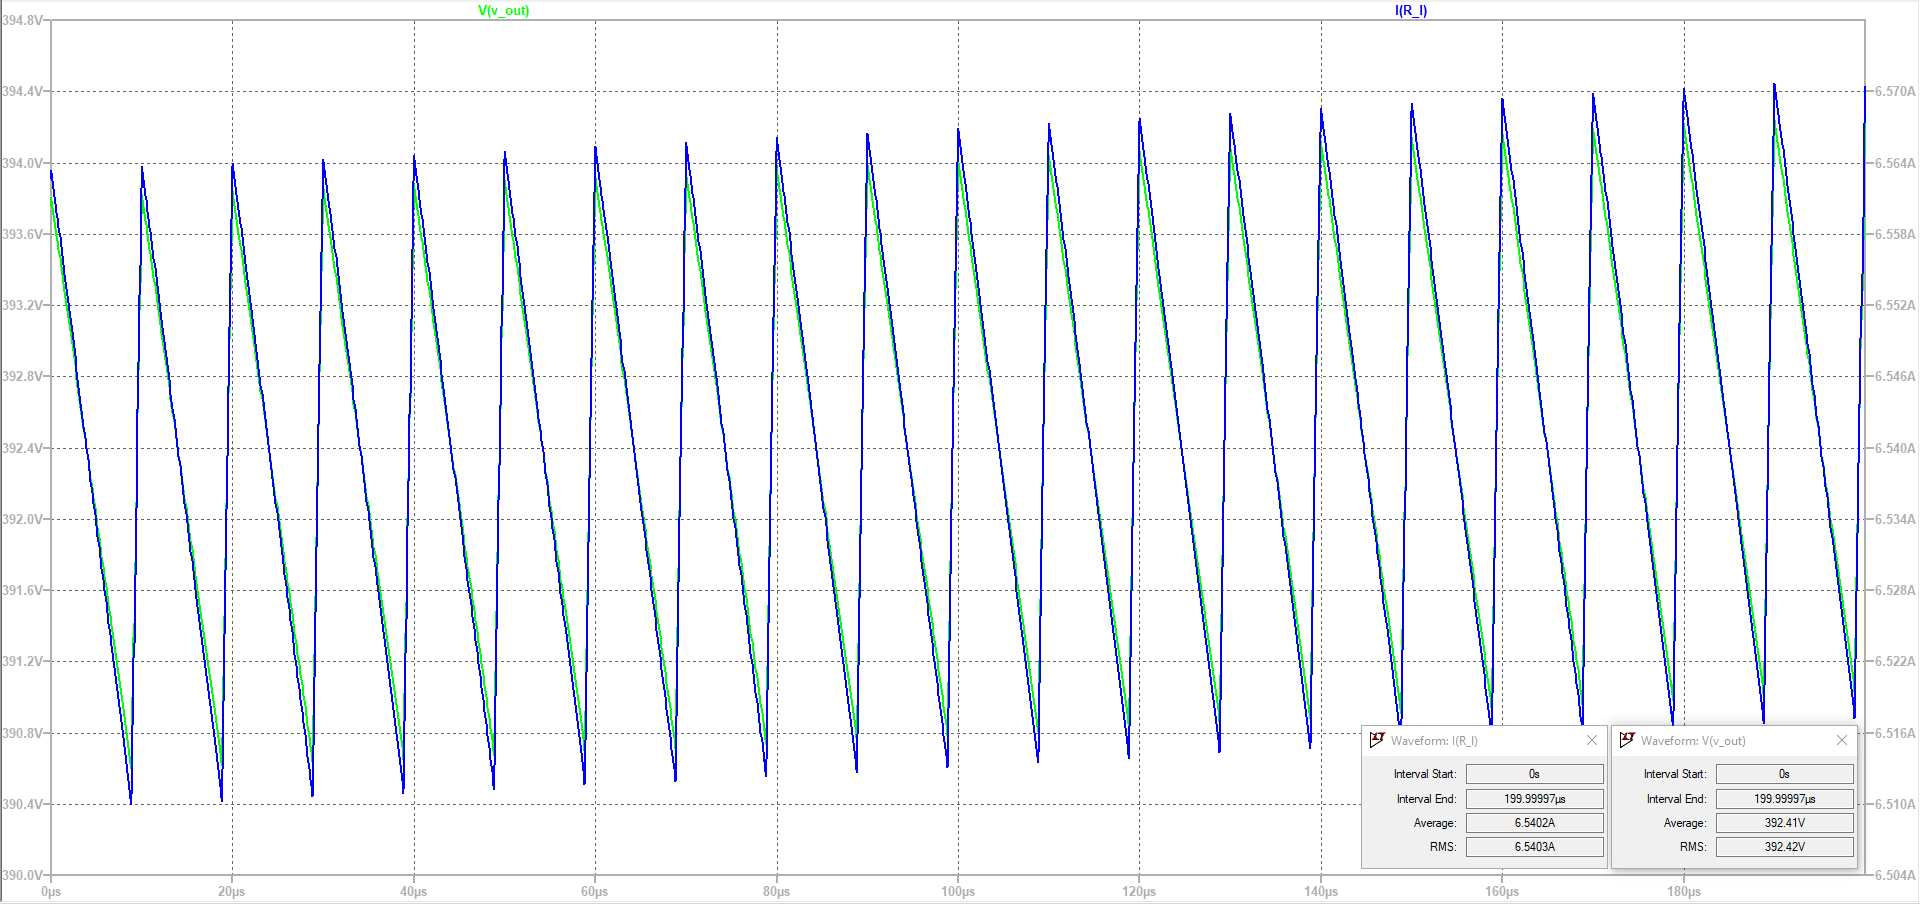
\includegraphics[width=1\linewidth]{Figura 9.png}
    \caption{Simulación en LTSpice del Convertidor Boost Monofásico. En \textcolor{green}{verde} se grafica la $V_{out}$ y en \textcolor{blue}{azul} se tiene la $I_{out}$.}
    \label{fig:fig_9}
\end{figure}

Se observa de los marcadores en la parte inferior derecha de la \autoref{fig:fig_9}, que el valor medio de la tensión es de: $V_{out(AV)} = 392.41 \ [V]$ y que el valor medio de la corriente es de: $I_{out(AV)} = 6.54 \ [A]$, siendo estos valores muy cercanos a los propuestos en el \underline{Paso 1} de la \autoref{sec_2.2.1} de modo que se valida el marco teórico empleado para desarrollar este convertidor. 

Resulta de interés también evaluar la similitud de las gráficas teóricas del \textit{Convertidor Boost} (Véase la \autoref{fig:fig_4}) con las que entrega el simulador, por lo que se realizan estas curvas en la \autoref{fig:fig_10} y la \autoref{fig:fig_11}.
\begin{figure}[H]
    \centering
    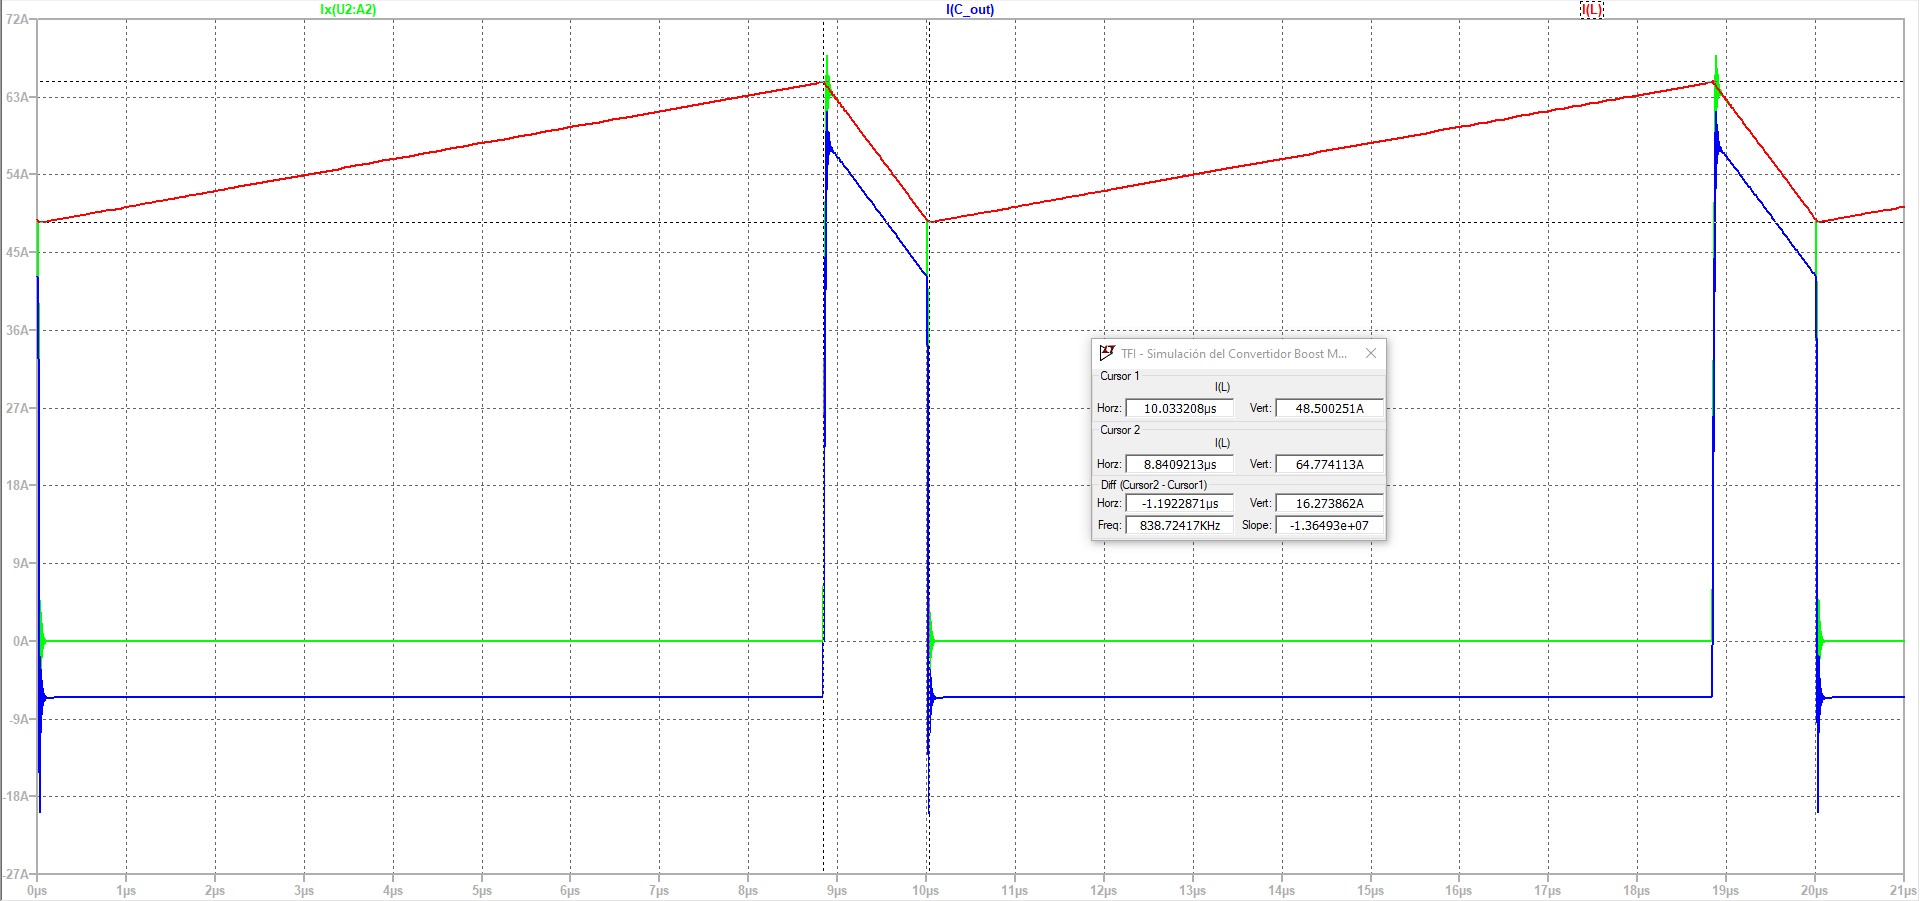
\includegraphics[width=1\linewidth]{Figura 10.png}
    \caption{Simulación en LTSpice del Convertidor Boost Monofásico. En \textcolor{red}{rojo} se grafica la $I_{L}$, en \textcolor{blue}{azul} se tiene la $I_{C_{out}}$. y en \textcolor{green}{verde} se grafica la $I_{D}$.}
    \label{fig:fig_10}
\end{figure}

Nótese que la diferencia entre la corriente más grande en $I_{L}$ (es decir: $I_{L(max)}$) y la corriente más chica (es decir: $I_{L(min)}$) se corresponde de forma directa al valor de $\Delta I_{L}$ el cual, según el marcador de la \autoref{fig:fig_10}, es igual a: $I_{L} = 16.27 \ [A]$ siendo este nuevamente un valor extremadamente próximo al encontrado en la \autoref{eq_14}.

Continuando con la comparativa de las curvas teóricas con las simuladas, también se observa de forma acertada en la \autoref{fig:fig_11}, que la Corriente del Inductor ($I_{L}$) es siempre la suma de la Corriente a través del Diodo ($I_{D}$) y la Corriente Drenador-Surtidor del \textit{MOSFET} ya que cuando conduce el Diodo, el \textit{MOSFET} estará apagado y cuando no conduce el diodo es porque el \textit{MOSFET} esta prendido.
\begin{figure}[H]
    \centering
    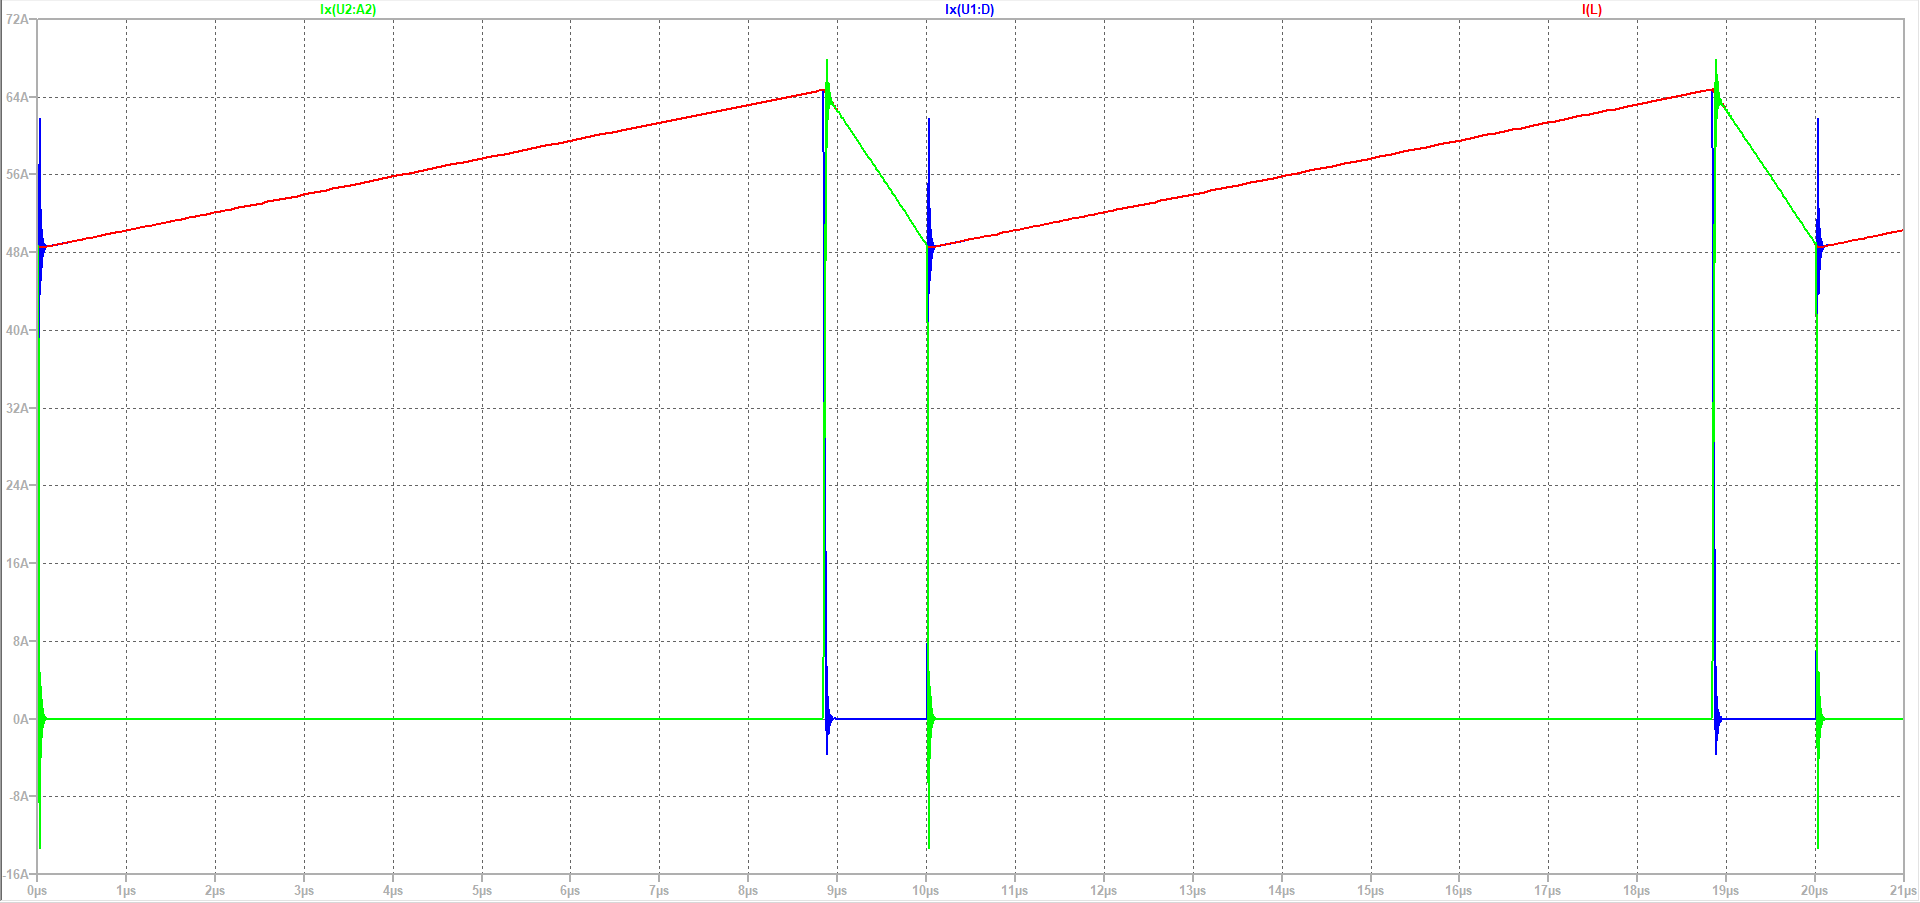
\includegraphics[width=1\linewidth]{Figura 11.png}
    \caption{Simulación en LTSpice del Convertidor Boost Monofásico. En \textcolor{red}{rojo} se grafica la $I_{L}$, en \textcolor{blue}{azul} se tiene la $I_{D}$. y en \textcolor{green}{verde} se grafica la $I_{D}$.}
    \label{fig:fig_11}
\end{figure}



\subsubsection{Simulación del Convertidor Boost Dual Trifásico}             \label{sec_2.2.4}
En virtud de lo expuesto en la \autoref{sec_2.2.3}, se tiene que el modelo empleado para el \textit{Convertidor Boost Monofásico} es válido y por lo tanto se busca en esta sección copiar ese esquemático y paralelizarlo de forma tal que se conforme el \textit{Convertidor Boost Dual Trifásico} que se desea investigar y desarrollar a lo largo de este informe.

Para poder observar una corriente de salida de: $I_{out} = 40 \ [A]$, se introduzco una resistencia de carga con valor igual al expresado en la \autoref{eq_24}.
\begin{equation}
    R_{L} = \frac{400 \ [V]}{40 \ [A]} = 10 \ [\Omega]
    \label{eq_24}
\end{equation}

Nótese que en este caso, ya no se simula un único \textit{MOSFET}, sino más bien 6 de ellos los cuales deben conmutar de forma intercalada, para evitar generar un cortocircuito. Para que el intercalado funcione y cancele el rizado de corriente, las 6 fases deben dispararse desfasadas exactamente $60 \ [\degree]$ una de otra ($360 \ [\degree] / 6 = 60  \ [\degree]$). Como el período total es de $10 \ [\mu s]$, el desfase en tiempo que debemos aplicar como retraso ($T_{delay}$) a cada fuente consecutiva es de:  $10 \ [\mu s] / 6 \approx 1.6667 [\mu s]$.


Por lo tanto, el circuito a simular es el que se muestra en la \autoref{fig:fig_12}:
\begin{figure}[H]
    \centering
    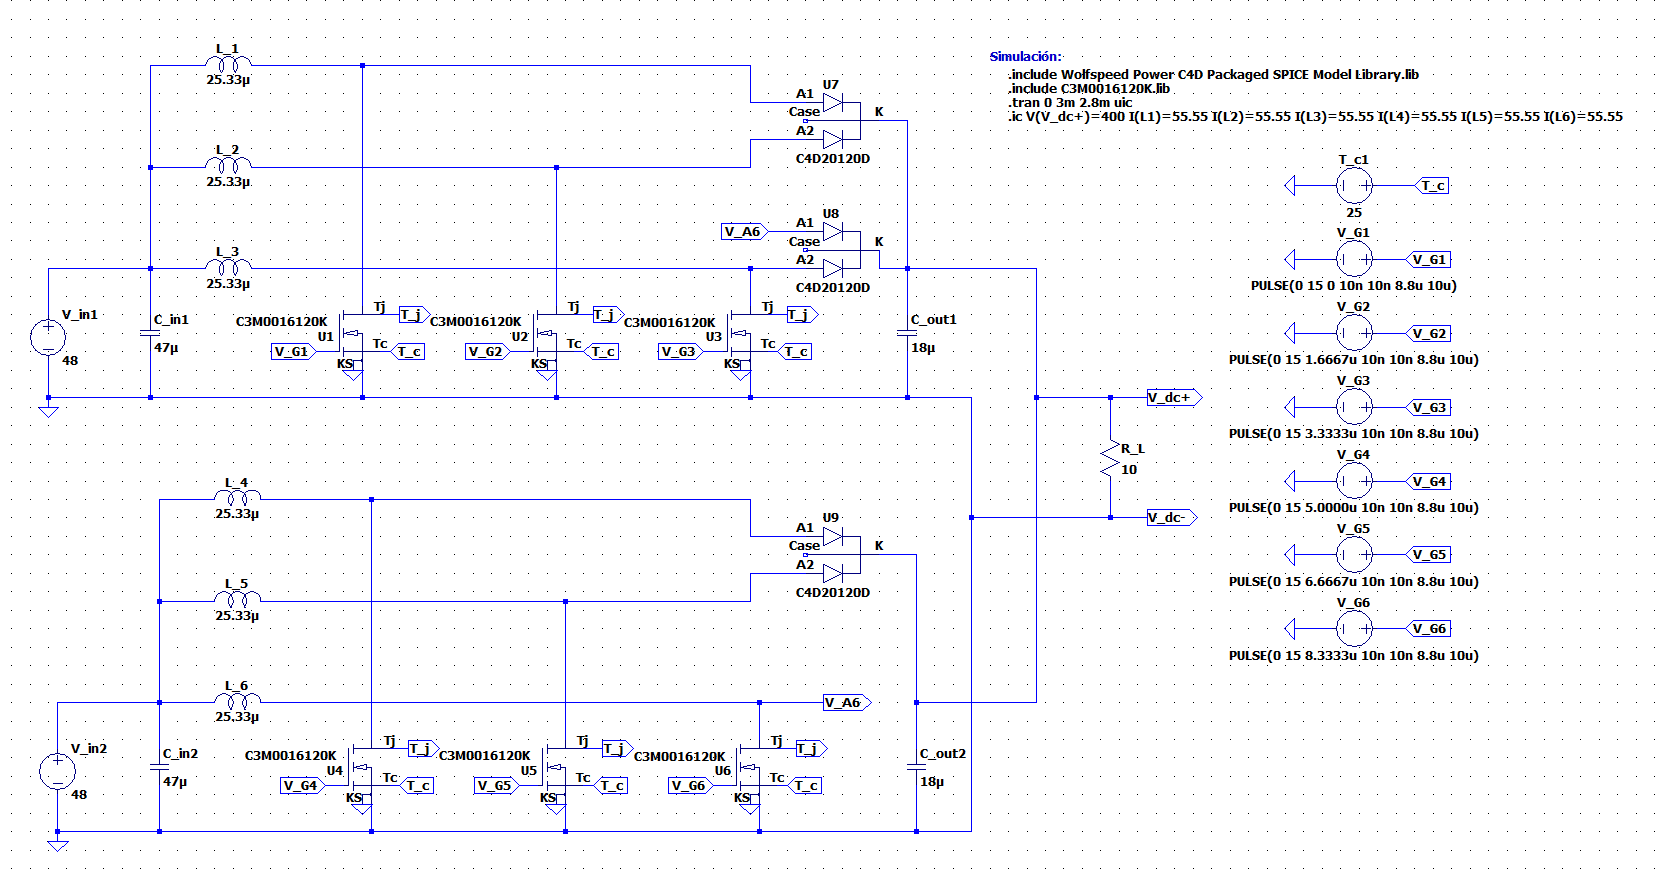
\includegraphics[width=1\linewidth]{Figura 12.png}
    \caption{Simulación en LTSpice del Convertidor Boost Dual Trifásico.}
    \label{fig:fig_12}
\end{figure}

Obsérvese que tal paralelización del circuito no es algo libre de consecuencias, ya que los modelos en LTSpice del Diodo y del \textit{MOSFET} provistos del fabricante \textit{Wolfspeed}, no son simples interruptores sino más bien subcircuitos altamente complejos, tal como muestra la extensa longitud de sus modelos en \autoref{anex_A} y \autoref{anex_B}. Estos subcircuitos incluyen un preciso modelado de las capacitancias parásitas dinámicas, resistencias no lineales y redes electro-térmicas acopladas (según los pines $T_{J}$ y $T_{c}$). Al simular 6 ramas operando a $100 \ [kHz]$, el motor de cálculo debe resolver extensos cálculos matemáticos con pasos de tiempo del orden de los nanosegundos para capturar correctamente las transiciones de encendido y apagado (pérdidas por conmutación), lo que eleva drásticamente el costo computacional.

Para mitigar los prolongados tiempos de simulación sin sacrificar la precisión del régimen permanente, se aplicaron 2 estrategias fundamentales de optimización:
\begin{itemize}
    \item \underline{Forzado de Condiciones Iniciales:} Se propuso que en lugar de simular el transitorio completo de carga de los Capacitores e Inductores (lo que llevaría un gran costo computacional), se opto por utilizar el comando $.ic$ (\textit{Initial Conditions}) para precargar los capacitores de salida a $400 \ [V]$ y que los inductores estén precargados con un determinado valor de corriente almacenado. Este valor de corriente se deduce partiendo de la \autoref{eq_24}.
    \begin{equation}
        P_{out} = \frac{V_{out}^{2}}{R_{L}} = \frac{400^2}{10} = 16000 \ [W]
        \label{eq_25}
    \end{equation}
    Dado que la potencia es constante, la corriente de entrada debe de ser igual a:
    \begin{equation}
        I_{in} = \frac{P_{out}}{V_{in}} = \frac{16000}{48} \approx 333.33 \ [A]
        \label{eq_26}
    \end{equation}
    Por lo tanto, la corriente por rama, y que consecuentemente debe tener el inductor en estado de régimen es de:
    \begin{equation}
        I_{L(rama)} = \frac{333.33}{6} \approx 55.55 \ [A]
        \label{eq_27}
    \end{equation}


    \item \underline{Agrupación mediante Módulos de Doble Diodo:} Nótese que el diodo \textit{Wolfspeed} $\ $ \textit{C4D20120D} consiste en único módulo con 2 diodos dentro del mismo, por lo tanto se tiene que 3 módulos ya sobrarían para modelar este circuito. Esta estrategia no sólo está justificada en la búsqueda de mejorar el rendimiento de la simulación, sino también en el objetivo de ahorrar espacio y compartir disipadores, permitiendo así reducir la cantidad de modelos térmicos independientes que el software debe evaluar simultáneamente y por lo tanto mejorando la convergencia sin alterar los resultados eléctricos del ripple de salida.
\end{itemize}

La elección de \textit{LTSpice} como software de simulación por sobre otros simuladores orientados a la electrónica de potencia es un planteo excede los propósitos de este Trabajo Final, sin embargo se propone revisar el \autoref{anex_C}, para justificar esta opción.

Con todo esto en mente, se puede realizar una simulación sobre la tensión y corriente de salida la cual se muestra en la \autoref{fig:fig_13}.
\begin{figure}[H]
    \centering
    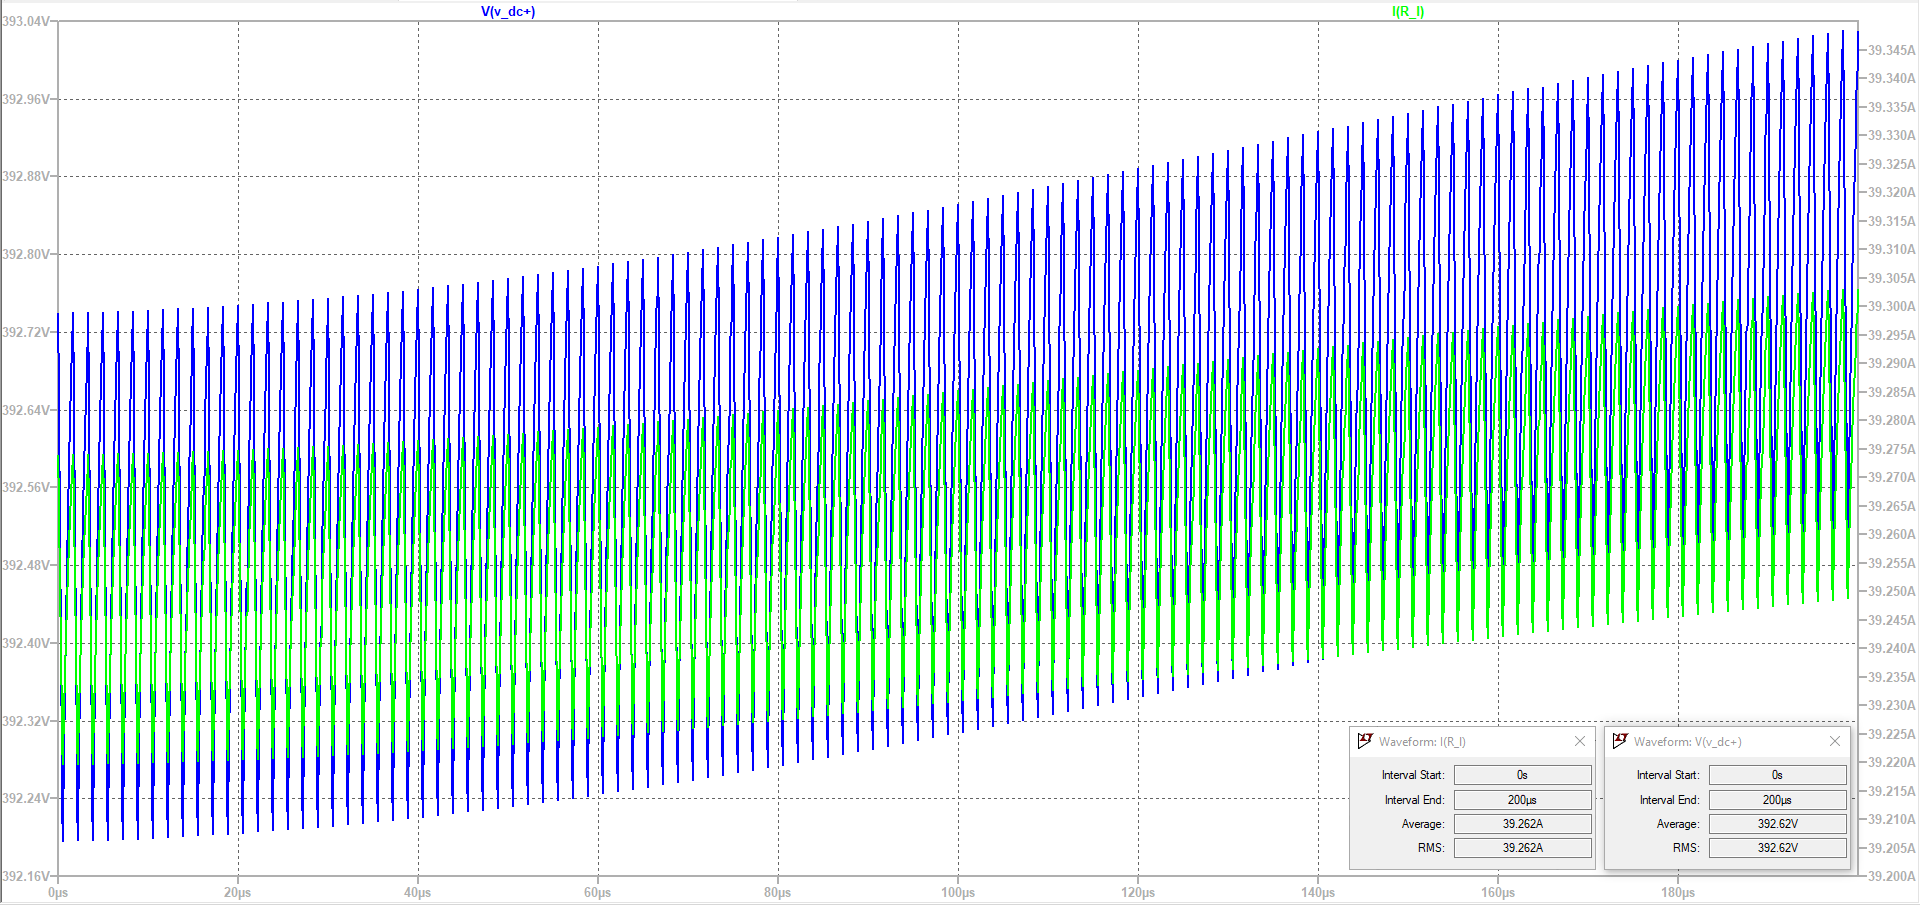
\includegraphics[width=1\linewidth]{Figura 13.png}
    \caption{Simulación en LTSpice del Convertidor Boost Dual Trifásico. En \textcolor{green}{verde} se grafica la $I_{out}$ y en \textcolor{blue}{azul} se tiene la $V_{out}$.}
    \label{fig:fig_13}
\end{figure}

Como podemos ver en la \autoref{fig:fig_13}, si bien en una primera vista parece que el sistema no ha llegado a su regimen, se tiene que al observar los ejes de tensión (a la derecha) y de corriente (a la izquierda), el valor de tensión media en la salida es de: $V_{out(AV)} \approx 392.62 \ [V]$ y la corriente media en la carga es de: $I_{out(AV)} \approx 39.262 \ [A]$. Nótese que estos valores son prácticamente los valores de diseño del \textit{Convertidor Boost Dual Trifásico}, verificando así el diseño y marco teórico desarrollado en apartados anteriores.

Se verifica tambien que el ripple de salida observado en la \autoref{fig:fig_14}, se corresponde a la $f_{efectiva}$ deducida según la \autoref{eq_15}, ya que $1/1.6666667 \approx 600 \ [kHz]$.
\begin{figure}[H]
    \centering
    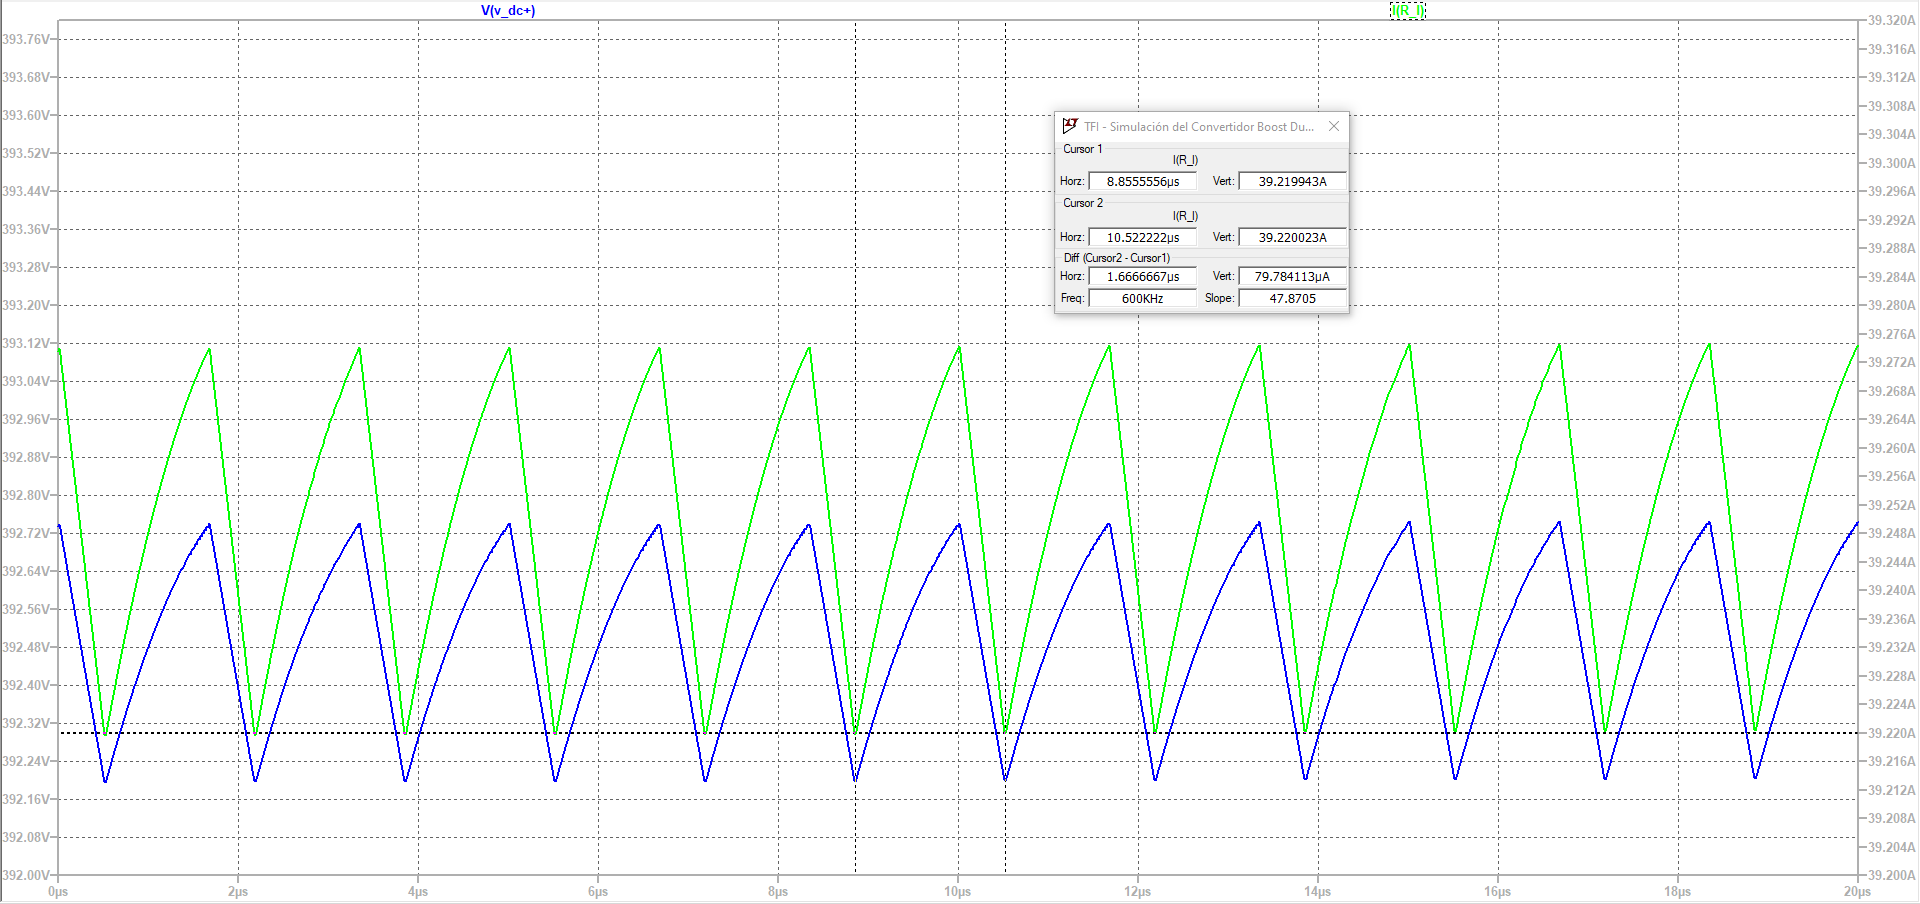
\includegraphics[width=0.95\linewidth]{Figura 14.png}
    \caption{Simulación en LTSpice del Convertidor Boost Dual Trifásico. En \textcolor{green}{verde} se grafica la $I_{out}$ y en \textcolor{blue}{azul} se tiene la $V_{out}$.}
    \label{fig:fig_14}
\end{figure}

Finalmente se muestra en la \autoref{fig:fig_15}, la corriente a traves de cada uno de los 6 Inductores que conforman el \textit{Convertidor Boost Dual Trifásico}, donde se observa que el valor medio de esta corriente es de: $I_{L} = 56.384 \ [A]$ que se aproxima al resultado obtenido en la \autoref{eq_27}.
\begin{figure}[H]
    \centering
    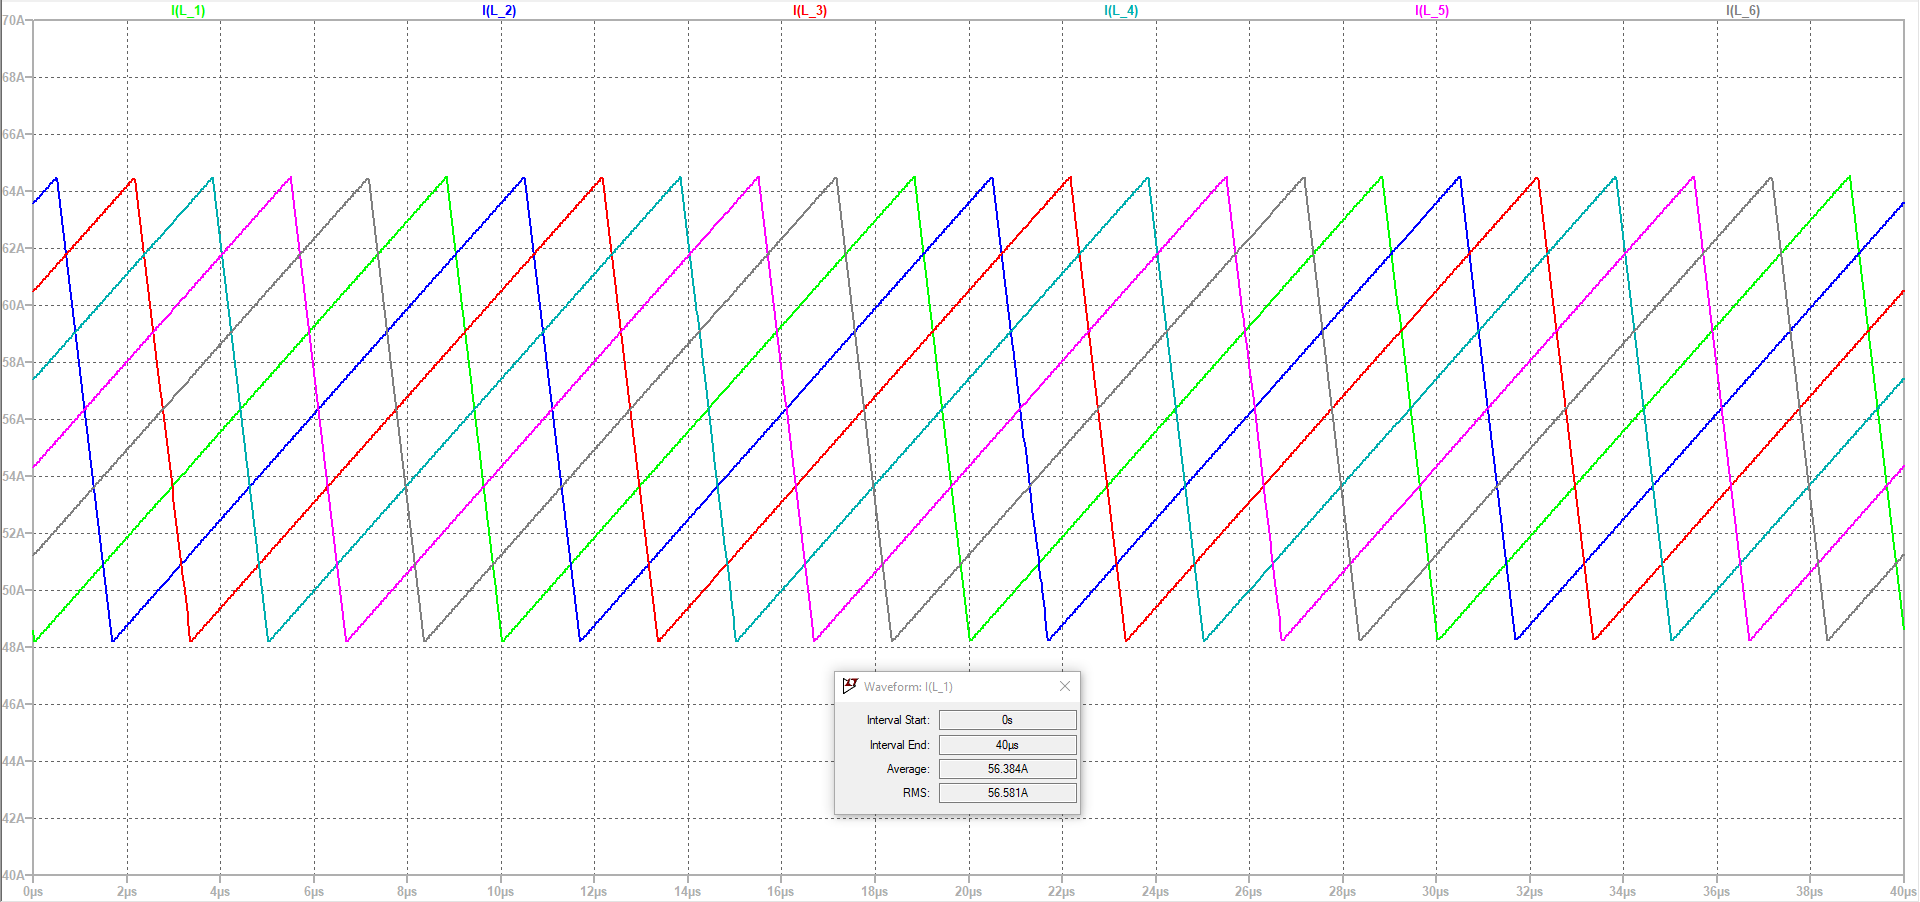
\includegraphics[width=0.95\linewidth]{Figura 15.png}
    \caption{Simulación en LTSpice del Convertidor Boost Dual Trifásico. En distintos colores se observan las distintas corrientes a través de los 6 Inductores.}
    \label{fig:fig_15}
\end{figure}



\subsection{Diseño del Circuito de Control}                                 \label{sec_2.3}
\subsubsection{Elección y Calculo del Circuito de Control}                  \label{sec_2.3.1}
Para la generación de pulso y el manejo de las compuertas de los \textit{MOSFETs} de \textit{SiC}, se descartó el uso de controladores analógicos tradicionales como el \textit{SG3525} ya que si bien son robustos, estos integrados están diseñados principalmente para topologías de 2 fases (\textit{Push-Pull} o Medio Puente) y carecen de la flexibilidad necesaria para generar 6 señales de pulso independientes con un desfase exacto de $60 \ [\degree]$. Además, su capacidad de entregar corriente (típicamente menor a $\approx 0.5 \ [A]$) resulta insuficiente para cargar rápidamente las capacitancias parásitas de un \textit{MOSFET} de \textit{SiC} operando a $f_{s} = 100 \ [kHz]$ \cite{b16}.

En virtud de lo expuesto, se optó por una arquitectura de control digital estándar en la industria actual:
\begin{itemize}
    \item \underline{Generación de señal digital ($MCU$/$DSP$):} Un microcontrolador se encarga de calcular el ciclo de trabajo y generar 6 señales lógicas (de $0$ a $3.3 \ [V]$) perfectamente sincronizadas y desfasadas para el disparo del \textit{MOSFET}.
    
    \item \underline{Etapa de Potencia de Compuerta (Gate Driver):} Nótese que los de $3.3 \ [V]$ y los pocos $[mA]$ de tensión y corriente de salida del microcontrolador, no pueden disparar el \textit{MOSFET} elegido. Por lo tanto se debe intercalar la salida del microcontrolador y la Gate del \textit{MOSFET} mediante un \textit{Gate Driver} en cada fase, el cual actúa como un amplificador que toma la débil señal digital del microcontrolador y la transforma en un pulso robusto de $15 \ [V]$, capaz de inyectar picos de varios amperios directamente en la compuerta del \textit{SiC}, garantizando una conmutación rápida y minimizando las pérdidas térmicas~\cite{b17}.
\end{itemize}


Se propone utilizar como microcontrolador un \textbf{TMS320F280049C} de \textit{Texas Instruments}, el cual es el estándar absoluto en cargadores de autos eléctricos y fuentes industriales. Tienen periféricos \textit{PWM} de muy alta resolución y están diseñados específicamente para manejar transistores de \textit{SiC}~\cite{b18}.

En cuanto al \textit{Gate Driver}, se propone utilizar un \textbf{LTC4440} de \textit{Linear Technology} el cual soporta una elevación de tensión de hasta $18 \ [V]$, lo cual será un margen más que suficiente para elevar los $3.3 \ [V]$ de salida del microcontrolador a la tensión de compuerta de: $V_{G} = 15 \ [V]$~\cite{b19}.



\subsubsection{Simulación del Circuito de Control con el Boost Monofásico}  \label{sec_2.3.2}
Se propone simular al microcontrolador elegido en la \autoref{sec_2.3.1} como una fuente de pulsos, ya que a fines prácticos: el microcontrolador, mediante una lógica programable interna, conmutará el estado de varios pines para generar los disparos. Nótese que intentar simular un microcontrolador dentro de \textit{LTSpice} es una tarea complicada la cual obviaremos si simulamos los pines de salida del micro como fuentes de pulso de tensión. La magnitud de los pulsos de tensión de salida se definen de acuerdo a la hoja de datos del \textbf{TMS320F280049C} de \textit{Texas Instruments}, la cual indica que las tensiónes de salida de los puertos \textit{I/O} son de $3.3 \ [V]$ \cite[Pág. 1]{b18}.

En cuanto al \textit{Gate Driver}, se tiene que el modelo elegido en la \autoref{sec_2.3.1} es nativo en \textit{LTSpice} y presenta una sencilla configuración tal como se muestra en la \autoref{fig:fig_16} para el \textit{Convertidor Boost Monofásico} con Circuito de Control.
\begin{figure}[H]
    \centering
    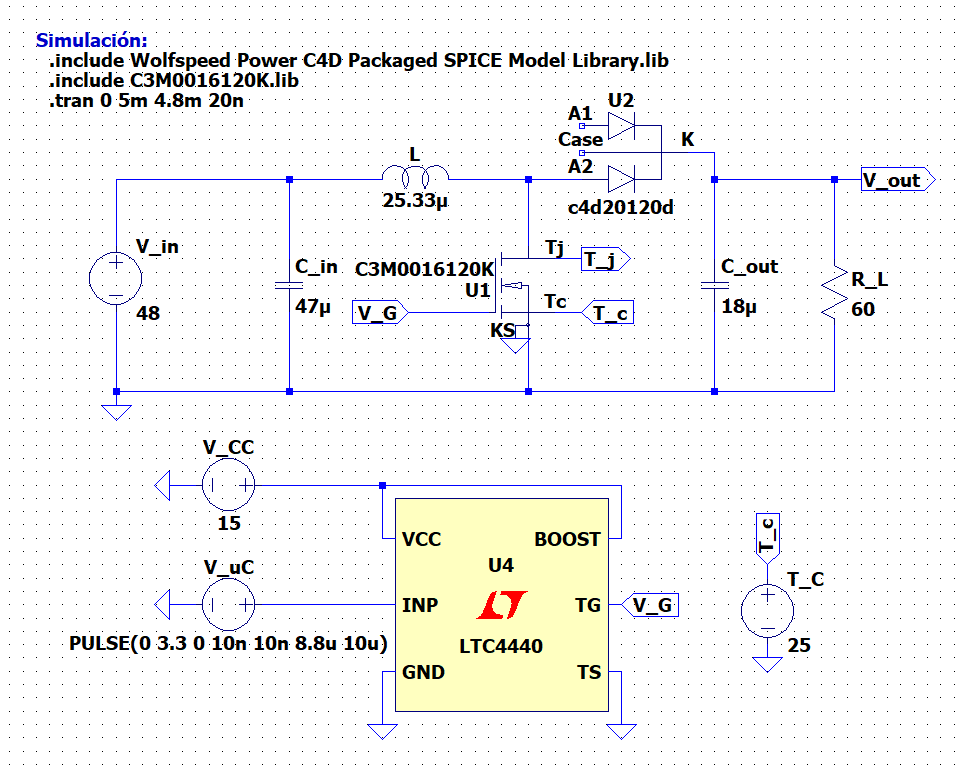
\includegraphics[width=0.6\linewidth]{Figura 16.png}
    \caption{Simulación en LTSpice del Convertidor Boost Monofásico con Circuito de Control.}
    \label{fig:fig_16}
\end{figure}

Al ejecutar la simulación, se puede observar que la tensión y corriente de salida son las que muestran la \autoref{fig:fig_17}.
\begin{figure}[H]
    \centering
    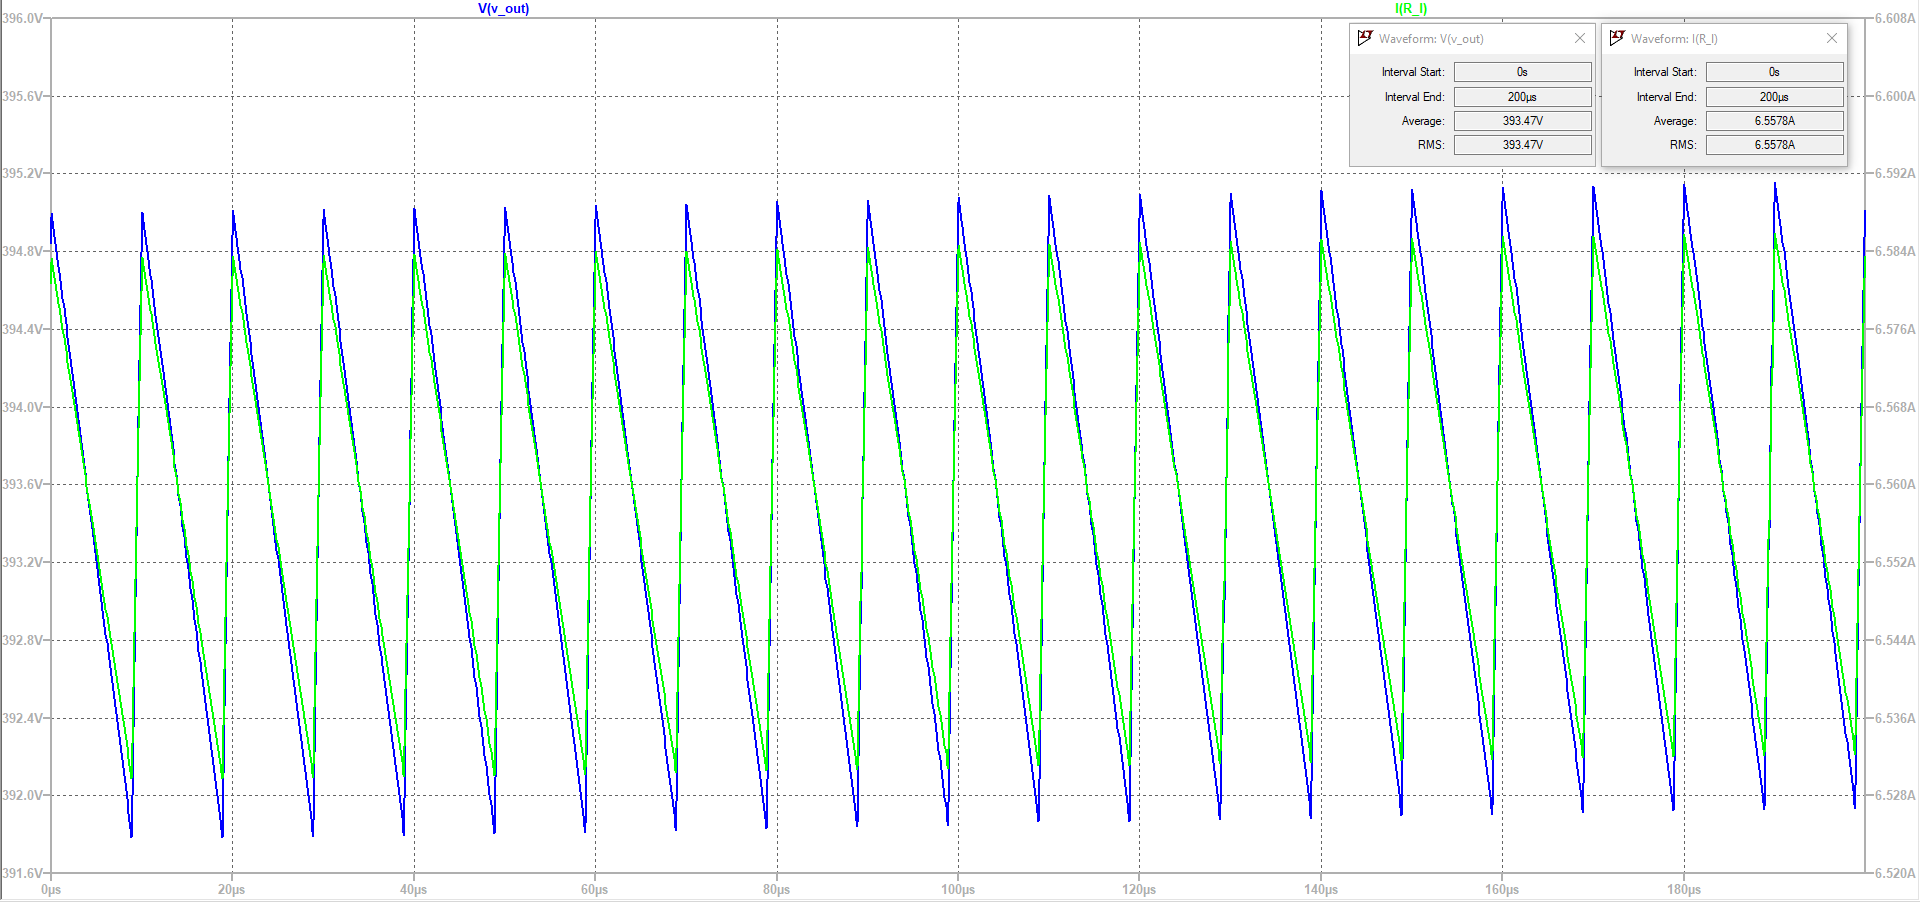
\includegraphics[width=0.95\linewidth]{Figura 17.png}
    \caption{Simulación en LTSpice del Convertidor Boost Monofásico con Circuito de Control. En \textcolor{green}{verde} se grafica la $I_{out}$ y en \textcolor{blue}{azul} se tiene la $V_{out}$.}
    \label{fig:fig_17}
\end{figure}

Nuevamente, los marcadores que se observan en la parte superior izquierda de la \autoref{fig:fig_17} indican que los valores obtenidos de tensión y corriente promedio de salida son los mismos que para el convertidor simulado sin circuito de control de la \autoref{fig:fig_9}, demostrando así el correcto funcionamiento del circuito de control en conjunto con el \textit{Convertidor Boost Monofásico}.




\subsection{Simulación Integradora y Análisis de Resultados}                \label{sec_2.4}
Para concluir este informe, se propone combinar el desarrollo de la \autoref{sec_2.2.4} del \textit{Convertidor Boost Dual Trifásico} sin circuito de control, con el desarrollo sobre el circuito de control de la \autoref{sec_2.3.2}, de modo que se obtiene una simulación final integradora del {Convertidor Boost Dual Trifásico} con un Circuito de Control tal como se ve en la \autoref{fig:fig_18}.
\begin{figure}[H]
    \centering
    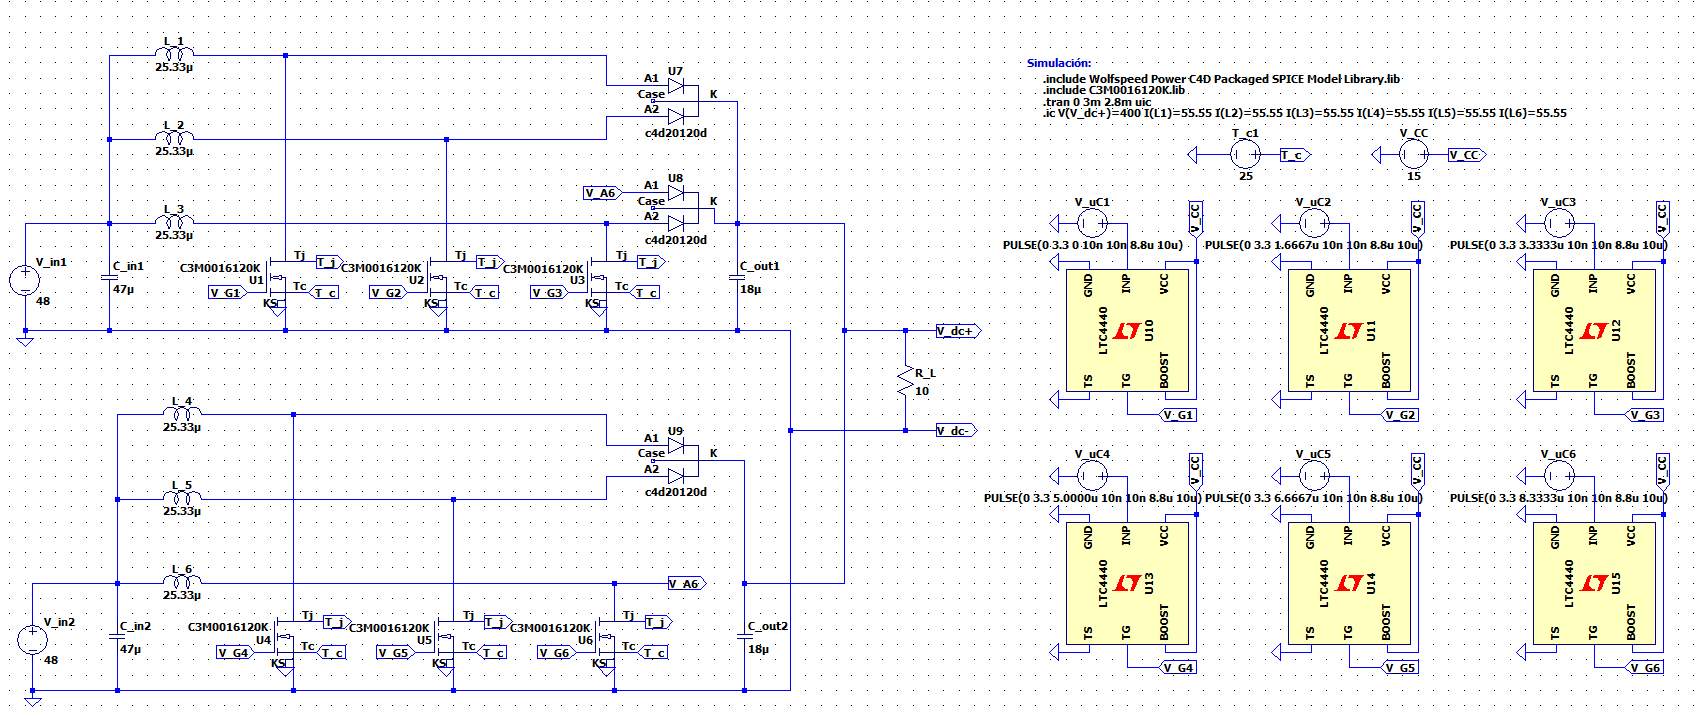
\includegraphics[width=1\linewidth]{Figura 18.png}
    \caption{Simulación en LTSpice del Convertidor Boost Dual Trifásico con Circuito de Control.}
    \label{fig:fig_18}
\end{figure}

Nótese que incluir a los 6 \textbf{LTC4440}, se relentiza aún más el proceso de simulación. Sin embargo, la simulación todavía puede ejecutarse de forma realista, y las curvas de salida son las que se muestram en la \autoref{fig:fig_19}.
\begin{figure}[H]
    \centering
    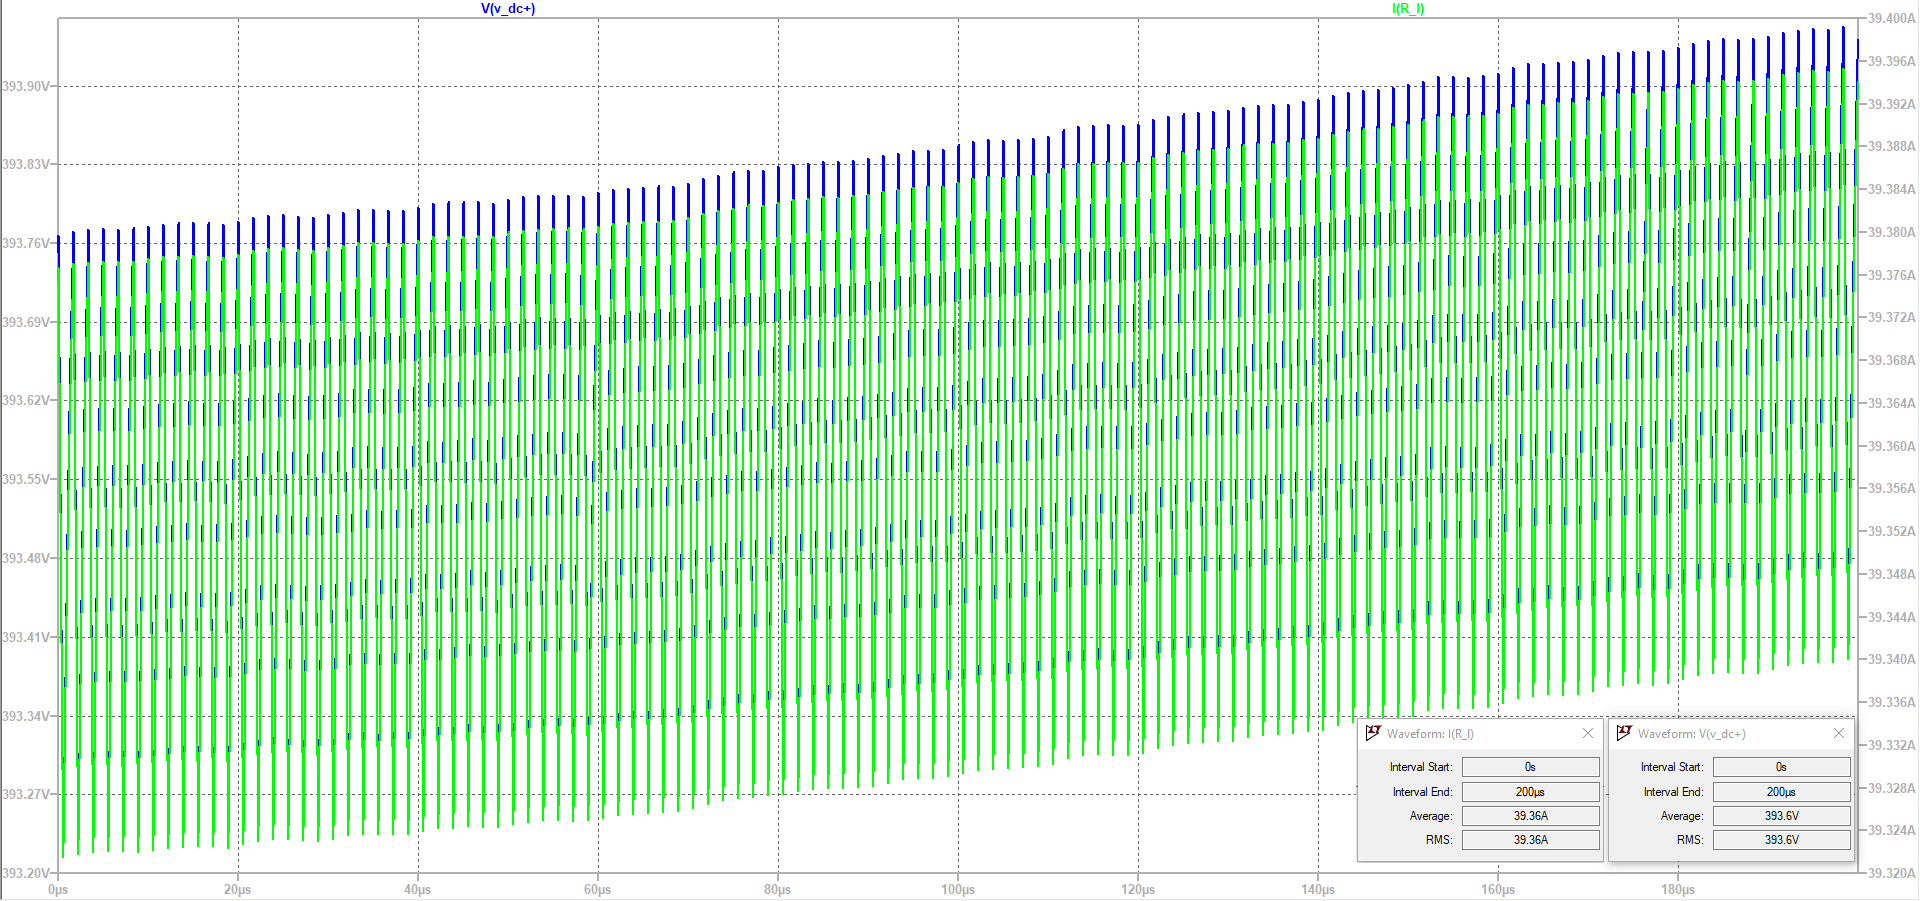
\includegraphics[width=1\linewidth]{Figura 19.png}
    \caption{Simulación en LTSpice del Convertidor Boost Dual Trifásico con Circuito de Control. En \textcolor{green}{verde} se grafica la $I_{out}$ y en \textcolor{blue}{azul} se tiene la $V_{out}$.}
    \label{fig:fig_19}
\end{figure}

Nótese que los valores nunca serán exactamente a los de diseño debido a errores de redondeo y ajuste de capacitores a valores comerciales, sin embargo los resultados obtenidos son, a fines prácticos, los mismos con los que se diseño el \textit{Convertidor Boost Dual Trifásico}, de modo tal que se concluye de forma exitosa que los objetivos propuestos en la \autoref{sec_1} han sido alcanzados satisfactoriamente y el circuito fue estudiado, analizado, diseñado y simulado correctamente. 





\section{Conclusiones}                                                      \label{sec_3}
\subsection{Conclusiones Técnicas}                                          \label{sec_3.1}
\begin{itemize}
    \item \underline{Validación del Marco Teórico:} A lo largo de este informe, se ha demostrado que el marco teórico utilizado para un \textit{Conversor Boost Monofásico} es un marco sólido para el diseño de este tipo de convertidores y que su análisis y diseño puede ser facilmente extendido a topologías de mas niveles en paralelo, como lo es la del \textit{Conversor Boost Dual Trifásico}. Este marco teórico también fue respaldado en base al simulador \textit{LTSpice}, el cual es una alternativa gratuita y de código abierto que presenta varias ventajas por sobre sus pares orientados a la electrónica de potencia tal como se discutión en la \autoref{anex_C}.

    \item \underline{Las ventajas de la Tecnología de \textit{SiC} en Aplicaciones Fotovoltaicas:} Esta tecnología representa un avance significativo a los diodos o \textit{MOSFETs} de \textit{Si} tradicional ya que permiten manejar altos valores de tensiones y corrientes mientras que pueden operar en un rango muy elevado de frecuencias. Esto los vuelve como una alternativa moderna y eficiente a la hora de diseñar circuitos convertidores \textit{DC-DC} para aplicaciones fotovoltaicas \cite{b12}.
    
    
    \item \underline{Complejidad en el \textit{Debugging} y Optimización de la Simulación:} El desarrollo del \textit{Conversor Boost Dual Trifásico} demostró que la optimización de una topología trifásica y dual presenta severas dificultades prácticas que escapan al análisis matemático ideal. El principal desafío técnico surgió durante la etapa de depuración (\textit{debugging}), donde se buscó realizar múltiples técnicas de optimización en el circuito para lograr compilar la simulación en un tiempo razonable y obtener los resultados de la simulación para verificar de forma veridica los resultados obtenidos.
\end{itemize}



\subsection{Conclusiones Personales}                                        \label{sec_3.2}
\begin{itemize}
    \item \underline{Valoración de las hojas de datos frente al diseño ideal:} Este proyecto nos permitió comprender de forma práctica que las ecuaciones de los libros de texto son solo el punto de partida para el diseño de circuitos. La ingeniería real exige un análisis aún más riguroso que el que proveen las hojas de datos de los fabricantes, ya que los límites físicos no lineales y las restricciones operativas de los componentes reales dictan la verdadera viabilidad y topología de un circuito electrónico, siendo este un concepto adquirido y profundizado a lo largo de esta asignatura.

    \item \underline{Fortalecimiento y Mejoras en el Proceso de Creación de un Informe Técnico:} A lo largo de los 10 \textit{TPTs} y este \textit{TFI}, propuestos por el Ing. Sergio Aguero, se buscó constantemente mejorar el proceso de análisis, diseño, optimización, obtención de material bibliográfico y demás procesos que fortalecen el crecimiento profesional de un Ingeniero. Dado que esta asignatura pertenece al último año de Ingeniería Electrónica de la \textit{FCEFyN}, se tiene que este informe ha sido de vital importancia para sentar las bases y comenzar el aprendizaje para un futuro proyecto de final de grado, independientemente si esta relacionado o no a la electrónica de potencia.
\end{itemize}



\newpage
\printbibliography[heading=bibintoc, title={4. \ Bibliografía}]             \label{sec_4}



\newpage
\appendix
\section{Modelo de LTSpice del Wolfspeed C4D20120D}                         \label{anex_A}
\begin{minted}[linenos]{bash}
********************************************************************************
** Wolfspeed SiC Schottky Diode C4D Family Spice Model Library
**     v1.3
** 01/26/2018
********************************************************************************
** Terms:
**	
** By using this SPICE Model (a "Model") from Wolfspeed, you on 
** behalf of your organization (or you personally, if you are requesting the 
** model for personal use) agree to the following conditions of its use:
**	
** 1. The Model, or any portion of the Model, is for your own use and may not 
** be distributed outside your organization (or to any other person or company,
** if you are acquiring the Model for personal use);
**	
** 2. You may use the Model only for the purpose of evaluating the performance 
** of Wolfspeed products in proposed circuits;
**	
** 3. The Model is provided “AS IS”, and Wolfspeed disclaims any warranty either 
** express or implied in connection with the Model, including but not limited 
** to any warranty
**	
** 4. In no event, will Wolfspeed be liable for any damages arising from the use 
** of the Model, regardless of the legal theory or any prior knowledge of Wolfspeed;
**	
** 5. Wolfspeed retains all copyrights and other intellectual property rights in 
** the Model. 
**	
********************************************************************************
********************************************************************************
** Notes:
** 1.  The model is designed to be accurate over the ranges presented in the
**     corresponding datasheet typical characteristic curves.
** 2.  The model is valid over the 25C to 175C temperature range.
** 3.  Reverse leakage currents are modeled as a breakdown voltage at 250uA.
**     No low current detail is provided.
** 4.  The surge response of the PiN structure is not included in this 
**     version.
** 5.  Recombination current is assumed to be zero.
** 6.  Currently, the model is electrical only. No thermal model is included.
** 7.  LT Spice users: please note that a LTSpice symbol library is also 
**     available. Please refer to the file "Wolfspeed_C4D_CPW4_LTSPICE_Symbols.zip" 
**     for further details.
**
********************************************************************************
********************************************************************************
** Release 1.3 notes
** 1.  Added all new TO-247-2 packages
**	
********************************************************************************
********************************************************************************
** Discrete Diodes
********************************************************************************
********************************************************************************
** TO-220-2 package
********************************************************************************

.subckt C4D02120A A K Case
L_anode		A	AD	6.5n
D1		AD	Case	CPW41200S002B	
L_cathode	K	Case	6.5n		
.ends

.subckt C4D05120A A K Case
L_anode		A	AD	6.5n
D1		AD	Case	CPW41200S005B	
L_cathode	K	Case	6.5n		
.ends

.subckt C4D08120A A K Case
L_anode		A	AD	6.5n
D1		AD	Case	CPW41200S008B	
L_cathode	K	Case	6.5n		
.ends

.subckt C4D10120A A K Case
L_anode		A	AD	6.5n
D1		AD	Case	CPW41200S010B	
L_cathode	K	Case	6.5n
.ends

.subckt C4D15120A A K Case
L_anode		A	AD	6.5n
D1		AD	Case	CPW41200S015B	
L_cathode	K	Case	6.5n
.ends

.subckt C4D20120A A K Case
L_anode		A	AD	6.5n
D1		AD	Case	CPW41200S020B	
L_cathode	K	Case	6.5n
.ends


********************************************************************************
**	TO-252-2 package
********************************************************************************

.subckt C4D02120E A K Case
L_anode		A	AD	6n
D1		AD	Case	CPW41200S002B	
L_cathode	K	Case	6n		
.ends

.subckt C4D05120E A K Case
L_anode		A	AD	6n
D1		AD	Case	CPW41200S005B	
L_cathode	K	Case	6n		
.ends

.subckt C4D08120E A K Case
L_anode		A	AD	6n
D1		AD	Case	CPW41200S008B	
L_cathode	K	Case	6n		
.ends

.subckt C4D10120E A K Case
L_anode		A	AD	6n
D1		AD	Case	CPW41200S010B	
L_cathode	K	Case	6n		
.ends


********************************************************************************
**	TO-247-2 package
********************************************************************************

.subckt C4D10120H A K Case
L_anode		A	AD	6.5n
D1		AD	Case	CPW41200S010B	
L_cathode	K	Case	6.5n
.ends

.subckt C4D15120H A K Case
L_anode		A	AD	6.5n
D1		AD	Case	CPW41200S015B	
L_cathode	K	Case	6.5n
.ends

.subckt C4D20120H A K Case
L_anode		A	AD	6.5n
D1		AD	Case	CPW41200S020B	
L_cathode	K	Case	6.5n
.ends



********************************************************************************
**	TO-247-3 package
********************************************************************************

.subckt C4D10120D A1 A2 K Case
L_anode1	A1	AD1	6.5n
D1		AD1	Case	CPW41200S005B	
L_anode2	A2	AD2	6.5n
D2		AD2	Case	CPW41200S005B	
L_cathode	K	Case	6.5n		
.ends

.subckt C4D15120D A1 A2 K Case
L_anode1	A1	AD1	6.5n
D1		AD1	Case	CPW41200S008B	
L_anode2	A2	AD2	6.5n
D2		AD2	Case	CPW41200S008B	
L_cathode	K	Case	6.5n
.ends	

.subckt C4D20120D A1 A2 K Case
L_anode1	A1	AD1	6.5n
D1		AD1	Case	CPW41200S010B	
L_anode2	A2	AD2	6.5n
D2		AD2	Case	CPW41200S010B	
L_cathode	K	Case	6.5n		
.ends

.subckt C4D30120D A1 A2 K Case
L_anode1	A1	AD1	6.5n
D1		AD1	Case	CPW41200S015B	
L_anode2	A2	AD2	6.5n
D2		AD2	Case	CPW41200S015B	
L_cathode	K	Case	6.5n		
.ends

.subckt C4D40120D A1 A2 K Case
L_anode1	A1	AD1	6.5n
D1		AD1	Case	CPW41200S020B	
L_anode2	A2	AD2	6.5n
D2		AD2	Case	CPW41200S020B	
L_cathode	K	Case	6.5n		
.ends


********************************************************************************

********************************************************************************
********************************************************************************


********************************************************************************
**	Die Models
********************************************************************************


.model CPW41200S002B			
+	d(		
+	level = 1
+	Is    = 6.99983E-13
+	N     = 1.320735113
+	Eg    = 1.251495861
+	xti   = 0.1
+	Rs    = 0.207862748
+	trs1  = 0.005385655
+	trs2  = 2.95075E-05
+	Cjo   = 1.65706E-10
+	VJ    = 1.127534358
+	M     = 0.458351103
+	bv    = 1697
+	tbv1  = 0.000744794
+	tbv2  = -7.92914E-06
+	tt    = 0
+	)		
		

.model CPW41200S005B
+	d(		
+	level = 1
+	Is    = 5.90598E-14
+	N     = 1.178186661
+	Eg    = 1.043467419
+	xti   = 7.950669626
+	Rs    = 0.098142507
+	trs1  = 0.004297495
+	trs2  = 2.59929E-05
+	Cjo   = 4.05432E-10
+	VJ    = 1.114512
+	M     = 0.467955771
+	bv    = 1639.597225
+	tbv1  = -0.00013199
+	tbv2  = -4.71787E-06
+	tt    = 0
+	)		
		

.model CPW41200S008B
+	d(		
+	level = 1
+	Is    = 1.92494E-14
+	N     = 1.11594604
+	Eg    = 1.035085337
+	xti   = 8.055126484
+	Rs    = 0.077114784
+	trs1  = 0.004446064
+	trs2  = 3.01628E-05
+	Cjo   = 5.56085E-10
+	VJ    = 1.441868153
+	M     = 0.487814696
+	bv    = 1566
+	tbv1  = 0.000611407
+	tbv2  = -6.93579E-06
+	tt    = 0
+	)		


.model CPW41200S010B
+	d(		
+	level = 1
+	Is    = 1.87454E-12
+	N     = 1.320015963
+	Eg    = 1.157943508
+	xti   = 4.026312737
+	Rs    = 0.050396905
+	trs1  = 0.005173515
+	trs2  = 2.80776E-05
+	Cjo   = 7.83471E-10
+	VJ    = 1.130882326
+	M     = 0.470404256
+	bv    = 1591.862027
+	tbv1  = 0.000157501
+	tbv2  = -5.61728E-06
+	tt    = 0
+	)		


.model CPW41200S015B
+	d(		
+	level = 1
+	Is    = 2.05199E-13
+	N     = 1.180245487
+	Eg    = 0.88047351
+	xti   = 12.65333425
+	Rs    = 0.042877267
+	trs1  = 0.004020008
+	trs2  = 2.59515E-05
+	Cjo   = 1.21052E-09
+	VJ    = 1.083744739
+	M     = 0.485774559
+	bv    = 1577.656188
+	tbv1  = -4.43126E-05
+	tbv2  = -7.15079E-06
+	tt    = 0
+	)		


.model CPW41200S020B
+	d(		
+	level = 1
+	Is    = 3.07768E-10
+	N     = 1.583842411
+	Eg    = 1.1120996
+	xti   = 5.433552149
+	Rs    = 0.028252912
+	trs1  = 0.005793999
+	trs2  = 2.29807E-05
+	Cjo   = 1.54979E-09
+	VJ    = 1.102078536
+	M     = 0.472648604
+	bv    = 1515
+	tbv1  = 0.001073165
+	tbv2  = -1.10208E-05
+	tt    = 0
+	)		
\end{minted}
~\cite{b20}



\section{Modelo de LTSpice del Wolfspeed C3M0016120K}           \label{anex_B}
\begin{minted}[linenos]{bash}
**************************************************************************************************************************************************************************************************
*
*     888888               888888 	        888888     .o888888888888o.     8888  		88888888888	o888888888888888     88888888888888o	88888888888   88888888888   8888888888o
*       88888             88888888             88888      .8888888  8888888.    8888  		88888888888    o8888888888888888     888888  8888888o	88888888888   88888888888   88888888888o
*        88888           8888  8888           88888      .8888888.  .8888888.   8888  		8888	       888888888	     888888  88888888	8888	      8888	    8888   88888
*         88888         8888    8888         88888       88888888    88888888   8888		8888   	       888888888	     888888  88888888	8888	      8888	    8888   88888
*	   88888       8888      8888       88888        88888888    88888888   8888  		8888888	       o888888888888888o     888888  8888888o	8888888	      8888888	    8888   88888
*	    88888     8888        8888     88888	 88888888    88888888   8888  		8888888		o888888888888888o    88888888888888o	8888888	      8888888       8888   88888
*	     88888   8888          8888   88888          88888888    88888888   8888  		8888		         88888888    8888		8888	      8888	    8888   88888
*	      88888 8888            8888 88888  	 .8888888.  .8888888.   8888  		8888 			 88888888    8888		8888	      8888	    8888   88888
*	       88888888	 	     88888888		  .8888888  8888888.    88888888888	8888		8888888888888888o    8888		88888888888   88888888888   88888888888o
*		888888		      888888  		   .o888888888888o.     88888888888	8888		888888888888888o     8888		88888888888   88888888888   8888888888o
*
*****************************************************************************************************************************************************************************************
** DISCLAIMER
********************************************************************************
** This model is provided as is, where is, and with no warranty of any kind
** either expressed or implied, including but not limited to any implied
** warranties of merchantability and fitness for a particular purpose.
********************************************************************************

********************************************************************************
** Wolfspeed SiC MOSFET C3M0016120K Spice Library
** Revision 1.0 Date: 05-17-2019
** Revision 2.0 Date: 11-12-2019
** Revision 3.0 Date: 08-12-2021
********************************************************************************
** Revision record
** Revision 1 Initial Release, Rev 04-2019
** Revision 2 Improved the accuracy of the IV curves
** Revision 3 Improved dynamic performance and updated parasitic inductance
********************************************************************************
** Parasitics Included
** Tj = Junction Temperature
** Tc = Case Temperature
** D = Drain
** G = Gate
** S1 = Kelvin Source
** S2 = Power Source
********************************************************************************

.subckt C3M0016120K d g s1 s2 Tj Tc
.param p11 = -8
.param p12 = 19
.param Rgint = 2.6

R1022 Tjc 0 1E6
E1022 Tjc 0 value {limit(v(Tj),-40,260)}

R100 gk s 1E6
E100 gk s value {limit(v(g1,s),-8,19)}

e33 NET3 0 Value {Limit(-93.938n*V(Tjc)**3+27.548u*V(Tjc)**2-5.5921m*V(Tjc)+
+                 2.6741,-1,3.5)}
R_cc NET3 0 1E6

xgmos d3 d1 gk s Tjc NET3 gmos_C3M0016120K

Ls1 s1 sv 5.17n Rser=8.4m
R_Ls1 s1 sv 100

Ls2 s2 sv 2.3n Rser=0.73m
R_Ls2 s2 sv 100

Rv sv s 100
Lv sv s 0.7n Rser=0

R_gg g1 s 1E6
R_g g1 g2 {Rgint}
Lg g g2 7.7n Rser=13.8048m
R_Lg g g2 100

Ld d d3 4.366n Rser=0.0874m
R_Ld d d3 8

Ed Id 0 value {I(Vdrain_s)}
Rdd Id 0 1E6

vdrain_s d3 d1 0
Gheat 0 Tj value = {abs((V(d1,s)*v(Id)))+abs((V(g1,g2)**2/Rgint))}

xCGD d3 g1 cgdmos_C3M0016120K
*CGS g1 s 6072p
CGS g1 s 6120p
xCDS d3 s cds_C3M0016120K

R15 dd12 d1 1E6
e15 dd12 d1 value {
+       if (V(gk,s)>V(NET3),
+       Limit(((881.9u*V(Tjc)**2+89.38m*V(Tjc)-34.9)*(V(gk,s)**3)+
+       (-25.75m*V(Tjc)**2-2.58*V(Tjc)+993.99)*(v(gk,s)**2)+
+       (0.16317*V(Tjc)**2+21.0784*V(Tjc)-6210.944)*v(gk,s)+
+       (-0.181*V(Tjc)**2-45.93*V(Tjc)+7848))/1000,-4,20)
+       ,
+       Limit(((328u*V(Tjc)**2+0.1011*V(Tjc)-33.982)*(V(gk,s)**2)+
+       (1.729m*V(Tjc)**2+0.98748*V(Tjc)-413.27)*v(gk,s)+
+       (15.27m*V(Tjc)**2-4.386*V(Tjc)-949.88))/1000,-4,5)
+       )
+}
vdiode1 dd12 dd14 0

Esn1 net1 0 value {I(vdiode1)}
Rsn1 net1 0 1E6

D1 s dd14 bodydiode_C3M0016120K 

CDS1 d3 s 0.1p
CGD1 g1 d3 0.01p
R_DS1 d3 s 0.5G

.model bodydiode_C3M0016120K d(is=0.88p bv=1590 n=4.80 T_abs=25
                             + rs=0.015 Tnom=25 tt=2n ibv=500u level=1)

R0 N1 Tj 41.15m
R1 N2 N1 90.58m
R2 N3 N2 47.43m
R3 Tc N3 91.1m

C0 Tj 0 2.803m
C1 N1 0 16.49m
C2 N2 0 42.52m
C3 N3 0 129.6m

*eth dd12d d1 value {1.145}

.ends C3M0016120K
********************************************************************************

.subckt gmos_C3M0016120K d3 d1 gk s Tjc NET3
e1 NET1 0 value {0.2}
R_A NET1 0 1E6

e2 NET2 0 Value {Limit(((-139.1u*V(Tjc)**2+10.05m*V(Tjc)+4.896)*v(gk,s)**2+
+               (4.183m*V(Tjc)**2-0.4445*V(Tjc)-55.01)*v(gk,s)+
+               (-30.04m*V(Tjc)**2+4.052*V(Tjc)+450.7))/
+               1000,0.01,2)
+               }
R_B NET2 0 1E6

e4 NET4 0 Value {Limit(((968.4u*V(Tjc)**2+32.99m*V(Tjc)-6.2299)*(V(gr)**2)+
+               (-22.807m*V(Tjc)**2-0.8652*V(Tjc)+111.88)*v(gr)+
+               (0.12453*V(Tjc)**2+5.5603*V(Tjc)-276.84))/1000,0,5)
+               }
R_d NET4 0 1E6

*e99 P99 0 value {0.02}
e9 P9 0 value {Limit(((-512.15u*V(Tjc)**2+0.16216*V(Tjc)-5.694)*(V(gr)**2)+
+             (10.273m*V(Tjc)**2-3.4705*V(Tjc)+109.74)*v(gr)+
+             (-37.963m*V(Tjc)**2+14.846*V(Tjc)-245.42))/1000,0.001,3)
+             }
R9 P9 0 1E6

*e6 NET6 0 Value {1.5}
e5 NET5 0 Value {Limit(((1.062u*V(Tjc)**2-360.348u*V(Tjc)-31.169m)*V(gk,s)**4+
+               (-62.037u*V(Tjc)**2+16.3645m*V(Tjc)+2.2536)*V(gk,s)**3+
+               (1.27528m*V(Tjc)**2-0.22406*V(Tjc)-54.823)*V(gk,s)**2+
+               (-10.06m*V(Tjc)**2+0.5774*V(Tjc)+490.499)*v(gk,s)+
+               (17.488m*V(Tjc)**2+4.4632*V(Tjc)-801.713))/1000,0.01,3)
+               }
R_e NET5 0 1E6

e10 NET10 0 Value {0.2}
R_K NET10 0 1E6

R1001 gr 0 1E6
E1001 gr 0 value {limit(V(gk,s),-8,15)}

e_P8 P8 0 Value {Limit((-613n*V(gk,s)**4+25.39u*V(gk,s)**3-
+               332u*V(gk,s)**2+1.726m*V(gk,s)-1.502m)*0.9,0.0001,0.1)
+               }
R_R P8 0 1E6

********************************************************************************
G2 d1 s value {
+   if(V(d3,s)<=0,
+       if (V(gk,s)<V(NET3),
+       0
+       ,
+       -((((v(NET5)+v(NET4))*(v(gk,s)-V(NET3))))*(1+v(P9)*v(s,d3))*
+       (((log(1+exp(v(gk,s)-V(NET3))))**2)- ((log(1+exp(v(gk,s)-V(NET3)-
+       (V(NET2)*v(s,d3)*((1+exp(-v(NET10)*v(s,d3)))**v(NET1))))))**2)))
+       *1
+       )
+       ,
+       if (V(gk,s)<V(NET3),
+       0
+       ,
+       ((((v(NET5))*(v(gk,s)-V(NET3))))*(1+v(P8)*v(d3,s))*(((log(1+
+       exp(v(gk,s)-V(NET3))))**2)-((log(1+exp(v(gk,s)-V(NET3)-
+       (V(NET2)*v(d3,s)*((1+exp(-v(NET10)*v(d3,s)))**v(NET1))))))**2)))
+       *1
+       )
+   )
+   }

.ends gmos_C3M0016120K
********************************************************************************

********************************************************************************
.subckt cgdmos_C3M0016120K d3 g1
.param k1=2565p
.param k2=0.5
.param ka=90
.param kb=0.3
.param kc=3.0

G11 g1 d11 value {
+   k1*(
+      (1+(limit(v(d3,g1),0.1,407))*(1+ka*(1+TANH(kb*V(d3,g1)-kc))/2))**(-k2)
+      )*ddt(v(g1,d11))
+   }
R_CGD d11 d3 1E-4
.ends cgdmos_C3M0016120K
********************************************************************************

********************************************************************************
.subckt cds_C3M0016120K d3 s
.param Cjo = 5179p
.param Vj  = 4.4365
.param M   = 0.643

G12 d12 s value {
+   (Cjo/(1+(limit(v(d3,s),0.1,580)/Vj)**M))*ddt(v(d12,s));
+   }
R_CDS d12 d3 1E-4
.ends cds_C3M0016120K
********************************************************************************
\end{minted}
~\cite{b20}



\section{Elección de LTSpice como Simulador de Circuitos}      \label{anex_C} 
Si bien en el ámbito de la electrónica de potencia existen simuladores especializados como \href{https://www.plexim.com/products/plecs}{PLECS} o \href{https://www.siemens.com/en-us/products/simcenter/systems-simulation/psim/}{PSIM} que destacan por su velocidad, estos suelen basarse en modelos de interruptores ideales o fuertemente simplificados, orientados al diseño de lazos de control. 

Los entornos como \href{https://www.plexim.com/products/plecs}{PLECS} o \href{https://www.siemens.com/en-us/products/simcenter/systems-simulation/psim/}{PSIM} operan bajo un paradigma de \textit{simulación sistémica}. En estos simuladores, los semiconductores son modelados macroscópicamente como interruptores ideales o cuasi-ideales. Las transiciones de conmutación se asumen instantáneas o lineales, y las pérdidas dinámicas o térmicas se estiman de forma retrospectiva utilizando tablas de búsqueda (Look-Up Tables) basadas en hojas de datos \cite{b21}. Si bien este enfoque es matemáticamente eficiente y resulta óptimo para el diseño de lazos de control cerrados de baja frecuencia, carece de la resolución necesaria para analizar fenómenos físicos de alta frecuencia en el lazo de potencia. Por el contrario, \textit{LTSpice} es un simulador de circuitos analógicos basado en la física del estado sólido. Su motor de cálculo resuelve ecuaciones diferenciales no lineales complejas en el dominio del tiempo continuo (con resoluciones del orden de los nanosegundos). Esto permite emular el comportamiento físico intrínseco del Carburo de Silicio (\textit{SiC}), incluyendo el proceso de carga y descarga de las capacitancias parásitas no lineales (\textit{efecto Miller}), las oscilaciones parásitas de alta frecuencia y las sobretensiones dinámicas originadas por las altas tasas de cambio de corriente y voltaje ($di/dt$ y $dv/dt$).

Dado que el objetivo crítico de esta etapa del diseño es verificar que los interruptores no superen su tensión de ruptura ($V_{DS(max)}$) durante las severas transiciones inducidas a $100 \ [kHz]$, el uso de \textit{LTSpice} resulta indispensable. Solo un análisis a nivel físico-microscópico permite garantizar la integridad eléctrica de los componentes frente a los transitorios destructivos que los simuladores sistémicos de interruptor ideal invisibilizan por completo. \cite{b21}

\end{document}